\documentclass[a4paper]{article}

%% Language and font encodings
\usepackage[english]{babel}
\usepackage[utf8x]{inputenc}
\usepackage[T1]{fontenc}

%% Sets page size and margins
\usepackage[a4paper,top=2.54cm,bottom=2.54cm,left=2.54cm,right=2.54cm,marginparwidth=1.75cm]{geometry}

%% custom packages
\usepackage{amsmath}
\usepackage{graphicx}
\usepackage[colorinlistoftodos]{todonotes}
\usepackage[colorlinks=true, allcolors=blue]{hyperref}
\usepackage{array}
\usepackage{multirow}
\usepackage{booktabs}
\usepackage{xcolor}
\usepackage{colortbl}
\usepackage{longtable}
\usepackage{lscape}
\usepackage{tikz-cd}
\usepackage{parskip}

%%special commands
\newcommand{\specialcell}[2][c]{%
  \begin{tabular}[#1]{@{}c@{}}#2\end{tabular}}
\newcommand{\invisiblesection}[1]{%
	\markright{#1}}
\newsavebox\tempbox
\newlength\templen

%%paragraph setup
%\setlength{\parskip}{1em}

\title{%
 Investor Sentiment and Stock Returns: \\
Wisdom of the Crowds }

\author{Linus Kinzel, Andrei Pauliuc and Imrich Valach}

\begin{document}
\maketitle

\vspace{30mm}
\begin{abstract}
\noindent Building on previous studies which prove that stock returns are influenced by investor sentiment, many authors have tried quantifying this relationship by employing traditional sentiment measures such as questionnaires and sentiment proxies. Although these approaches provide fairly reliable measures of investor sentiment, recent technological developments have presented us with new tools which help in measuring investor sentiment in faster and more novel ways. Social platforms for investors and natural language processing algorithms categorizing Tweets are two of such tools. Using a modern approach, the aim of this paper is to analyse how investor sentiment measured by these new instruments can help in predicting subsequent stock returns. After an evaluation of the current state of research on this topic, we describe our big data centric research design and the sentiment and stock data used in this research. The results of the regression analyses confirm the existence of the relationship; on top of that, these relationships are negative for short time lags of one week and one month, but positive for longer lags. In addition, we find positive associations between traditional and modern sentiment measures. Therefore, these new measures provide not only a reliable, but also a faster method of quantifying investor sentiment.
\end{abstract}

\vspace{70mm}
\invisiblesection{disclaimer}
\textit{This paper is written by Linus Kinzel, Andrei Pauliuc and Imrich Valach, who take full responsibility for its contents. We declare that all text is our own work and no other sources have been used except the ones present in the bibliography. RSM is only responsible for supervision of completion of the work but not for its contents.}

\newpage
{\parskip=0pt
\tableofcontents
}

\section{Introduction and Theory}

The efficient market hypothesis, which is predominantly taught in university level finance courses, argues that stock markets are efficient in such a way that the current price of a stock always incorporates all known information. This implies that stocks are always priced at the monetary value of their actual worth (Fama 1965). Moreover, it means that reaping abnormal returns over continued time periods is not possible, because as soon as information affecting the value of a stock becomes available, it is already reflected in its price. While the efficient market hypothesis is an excellent way of introducing students to the way financial markets work, the history of stock markets quickly reveals that there are frequent occurrences where the theory falls short in explaining the movements of the market. The most vivid examples are booms, bubbles and crashes, such as the Great Crash of 1929 or the dot-com bubble of the late 1990s. The high volatility throughout such events illustrates that the stocks cannot constantly carry their actual, reasonable value. 
\par
Behavioural finance delivers an alternative view on the matter. It acknowledges that the part of the market which is still run by humans, not machines, is prone to human error and emotions such as investor sentiment. While the efficient market hypothesis was developed in the 1960s and has been popular since then, from the late 1980s onward a different perspective emerged and evolved, employing behavioural finance to find reasons behind extreme market movements. It seems the key event here was the stock market crash of 1987.  Delong, Shleifer, Summers, and Waldmann (1990) established the existence of investor sentiment, thereby paving the way for a series of studies on investor sentiment in the coming decades. 
\par
Investor sentiment can either be bearish, neutral or bullish - bearish is a weak investor sentiment; bullish is a strong investor sentiment, meaning that investors believe that the stock market will see price increases in the foreseeable future. Fisher \& Statman (2000) were among the first to establish that investor sentiment is commonly a contrarian indicator, meaning that a bullish sentiment is often followed by falling stock prices. The rationale behind this is that bullish sentiment often causes an overreaction by traders and lifts stock prices above the fundamental value of the stock (Barberis et. al 1998). When the market adjusts, stock prices fall. The inverted case of bearish sentiment and subsequent gains take place in similar, yet opposite fashion. Negative sentiment, built up in interaction with overreaction to negative news, causes immediate diminishing returns but in the short to medium-term drives prices upward during the adjustment.
\par
Going back to the roots of sentiment research, Baur et al. (1996) established that fundamentals, not sentiment, were behind the driving force behind market movements around the crash in 1987, but Shleifer \& Vishny (1997) found that betting against sentimental investors is risky and can be costly. Next, Neal \& Wheatley (1998) drew the connection between sentiment and stock returns by analysing the correlation of different sentiment measures and subsequent stock returns, and found that some of their implicit sentiment measures have a negative relationship to stock returns.
\par
In the 2000s, researcher developed a consensus about investor sentiment. The existence and the relation to stock returns were mostly undisputed. Thus, researchers focus shifted towards the circumstances under which the prediction value of sentiment regarding stock returns is especially valuable. Baker \& Wurgler (2007) state that stocks which are difficult to value or arbitrage are especially vulnerable to mispricing because of investor sentiment. This seems in line with the idea of placing sentiment as one of the reasons behind crashes: the dot-com bubble, for example, consisted of numerous overvalued start-up firms which are naturally hard to assess in their value, because valuations are calculated in terms of insecure future earnings. Schmeling (2007) added to this distinction behind stocks that not only the stock type makes a difference, but also the investors themselves. The sentiment of individual investors as well as investors in country-cultures with herd-like behaviour are more prone to overreaction and therefore have a higher sentiment and return correlation.
\par
The prediction value of sentiment is relevant for researchers as well as managers. If sentiment is the underlying cause of market crashes, sentiment knowledge may reduce extents of cash-destroying market movements. On a smaller scale, sentiment knowledge can support managers in assessing the risk of stock prices which are not based on fundamentals. Unfortunately, prior research inhibits some disagreements regarding the prediction value of sentiment for stock returns. Brown \& Cliff (2002) see little predictive power of investor sentiment for future returns, whereas Fisher \& Statman (2000) go as far as claiming that investor sentiment can be used in a tactical asset allocation programme. 
\par
To bring more clarity around this topic, our research investigates the following central hypothesis: Increases in investor sentiment are related to subsequent decreases in stock prices. With this hypothesis, the goal is to determine if stronger investor sentiment is followed by declining stock prices, as well as the strength of the decrease. This yields the following research question:

\vspace{10pt}
\begin{center}
\parbox{375pt}{ \centering
\textit{Is there a negative relationship between investor sentiment and stock market returns? If yes, how much prediction value does sentiment carry?}
}
\end{center}
\vspace{10pt}

While measuring stock returns is straightforward, correctly identifying and magnifying investor sentiment is a trickier undertaking. There are two distinct approaches. More common are sentiment surveys directly sent out to investors, such as the survey by American Association of Individual Investors (AAII). However, indirect attempts are utilized as well, such as proxying the consumer confidence index into investor sentiment (Schmeling 2009) or the first day returns during IPOs (Baker \& Wurgler 2006).  Investor sentiment is usually grouped by different types of investors, such as small-volume hobbyists or professional Wall Street investors. 
The dependent variable is stock market returns. Returns are the gains a specific stock achieved over a period of time, and can theoretically be measured on any stock, making the focal unit of our research the stock market in general. The main features of the research are summarised in Table~\ref{tab:research_features} below:

\begin{table}[h]
\centering
\begin{tabular}{>{\bfseries}l | r}
Focal Unit & Stock Market \\\hline
Theoretical Domain & All stock markets in all countries at all times\\\hline
Independent variable & Investor Sentiment\\\hline
Dependent variable & Stock returns\\\hline
Causal Relationship & Causal, probabilistic, negative
\end{tabular}
\caption{\label{tab:research_features}Research features}
\end{table}

\[
	\begin{tikzcd}
    Investor Sentiment \arrow{r}{-} & Stock Returns
	\end{tikzcd}
\]
\par 
In this paper, we will focus on the indicated unidirectional, negative relationship. Causality in investigating the relationship of investor sentiment and subsequent stock returns can be implied for multiple reasons: past papers, which established the existence of the relationship, applied time lags and applicable causality tests. Furthermore, there is economic theory behind the causality as well.  As mentioned, bullish sentiment often creates an overreaction by traders which lifts the stock price momentarily above its real value, but forces prices to fall after an appropriate time period has passed. For bearish sentiment the opposite chain reaction ensues.
\par
These are the cornerstones of our research. In the next chapter of this paper, Section~\ref{critical-evaluation},  we will introduce a set of articles with similar research objectives and thereby create an overview of the current state of research. We will analyse the quality of these papers in terms of their research strategies and variable measurement techniques. Section~\ref{criticalsynthesis} finalizes the literature review by comparing the effect sizes of the articles, i.e. examining the strength of the sentiment-returns relationship. Section~\ref{research-proposal-section} lays out the structure of our own research and, afterwards, we present its results in Section~\ref{results-section}. Finally, we provide a detailed discussion of these results and present our conclusions in Section~\ref{discussion-section}.

\section{Critical Evaluation} \label{critical-evaluation}

\subsection{Introduction and Article Selection}
Even though the current literature on investor sentiment and stock returns employs a wide spectrum of methodologies and produces volatile results, the outcomes seem to incline towards the notion that investor sentiment negatively influences subsequent stock returns. This section presents an analysis of a comprehensive set of prior studies. The studies are carefully selected on the criteria of being strongly related to our hypothesis, the significance of their results and the appropriateness of methodologies used. Articles with wide range of different measures are analysed to gain insights on their applicability, validity and reliability.

\subsection{Hypotheses and Methodology}
As indicated above, even though most of the research mainly centres on investigating the influence of investor sentiment on the stock market returns, the exact methods and focus differ. Smales (2017), Neal and Wheatley (2001), Brown and Cliff (2002), Schmeling (2009) and Baker and Wurgler (2007) approach the research in a similar manner and employ the general hypothesis:  higher (lower) investor sentiment decreases (increases) stock returns. Some authors focus on individual investors only (Kumar and Lee 2002), test for non-linear relationship (Dergiades 2012) or the effect of recession and expansion on the relationship between sentiment and returns (Chung et al. 2012). Furthermore, there are differences in geographical location, the size of the firms analysed and time lag between measuring sentiment and stock returns. The following section summarizes the hypotheses and methodologies and compares the different approaches. The results of the studied literature are in Section~\ref{criticalsynthesis}, Critical Synthesis.

\paragraph{Geographical Location}
The articles focus mainly on US stock markets (NASDAQ and NYSE) where they also draw the stock returns data from. Schmeling (2009), however, investigates the effect of investor sentiment in 18 countries (including US) by employing consumer confidence as the sentiment proxy. This is in contrast with research conducted solely in the US, which mainly uses surveys or newsletters. Next to the general hypothesis, Schmeling (2009) also investigates hard-to-value stocks and the effect of market institution development and culture on the relationship between investor sentiment and stock returns. The paper tries to improve understanding of the source of investor sentiment (such as investor overreaction) by connecting Hofstede's (2001) findings. As such, the paper investigates whether cultural differences might play a role in behavioural biases. Chui et al. (2008) argue that investors in countries with high scores on collectivism are more prone to be influenced by the crowd and thus the connection between sentiment and returns is expected to be stronger.

\paragraph{Type of Firm}
Similar to Schmeling (2009), the second hypothesis of Smales (2017) aims to investigate whether small, hard-to-value firms react stronger to sentiment. This also applies to Brown and Cliff (2002), Fisher and Statman (2000) and Chung et al. (2012). The authors divide the companies based on book-to-market ratio and returns (Smales 2017), or the Center for Research in Security Prices' (CRSP) deciles and NYSE breakpoints. The papers differ in the use of CRSP deciles. CRSP deciles are companies divided into groups based on market capitalization.  The largest companies are in decile 1 and the smallest companies are in decile 10. For Fisher and Statman (2000), the small stocks are in deciles 9-10 whereas Brown and Cliff (2004) uses CRSP deciles 6-8. As largest stocks, they employ the largest quintile of NYSE/AMEX/NASDAQ. All the authors predict that stock returns of smaller firms are more likely to be influenced by investor sentiment as there is not enough information and thus the hard-to-value stocks are hard to arbitrage.

\paragraph{Recession and Expansion}
Chung et al. (2012) and Smales (2017) investigate the influence of recession and expansion of the economy state on the relationship between investor sentiment and stock returns. Both papers employ monthly sentiment measures and determine the state of economy based on data by the National Bureau of Economic Research (NBER). Chung et al. (2012) also use Markov switching models to determine what is the state of economy. Smales (2017) aims to investigate whether fear, represented by the Volatility Index (VIX), or confidence (Consumer Confidence Index) is better at predicting stock returns. Behavioural argumentation suggests that fear should be a better predictor, as people are more responsive to fear compared to confidence. This implies that during recession, investor sentiment should be more predictive of subsequent stock returns. 

\paragraph{Short-Term versus Long-Term}
Regarding the time frame and duration of the lags, the hypotheses of the authors test that the effect of investor sentiment is diminishing over time. This is a result of additional events affecting the market and changing the sentiment of investors. Subsequently, the investors are likely to adapt their strategy to this new information (Brown and Cliff 2005). Fisher and Statman (2000) investigate only one month lag periods whereas Schmeling (2009) looks at 1, 6, 12 and 24 months lag periods. Brown and Cliff (2002) also investigate weekly next to monthly periods. In multiple articles, the choice of the lag periods is influenced by the availability of investor sentiment data. This applies especially for international research conducted by Schmeling (2009). 

\paragraph{Individual vs Institutional}
Institutional and individual investors' investing strategies are diametrically different: the former as a profession, the latter mainly as a source of income alongside his professional job. This influences the behaviour of the distinct groups. Individual investors trade much less often, spend less time on investment analysis and rely on different sources of information than institutional investors do. Kumar and Lee (2003) aim to investigate the origins of the investor sentiment as they feel that most past studies tried to document only the mere existence of investor sentiment. 
\par
In their article, they find that individual investors tend to be more prevalent in the decile-9 stocks (small stocks – in the ninth decile of NYSE by market capitalization). Furthermore, they argue that the relative scarcity of publicly available information for smaller firms may induce individual investors to seek advice from investment newsletters. As a result, the activity around small stocks is largely influenced by the sentiment of investment newsletters (as the individual investors seek advice from this source and they are most prevalent in the segment of small stocks). In conclusion, individual investor sentiment tends to influence small stocks, value stocks, stocks with low institutional ownership and stocks with lower prices. In Fisher and Statman (2000), we can see that the sentiment of institutional investors and individual investors is not correlated at all (0.01). This underlines the information asymmetry, as well as the irrationality, which is likely to be exhibited to a larger extent by individual investors rather than Wall Street strategists.

\subsection{Research Strategies}
The different methodologies discussed above are implemented into very similar research strategies. The researchers conduct panel studies which are quasi-experimental. Panel studies are used when the variables are continuous and not binary (present/non-present). They have lower internal validity than experiments. However, in stock market research, experiments are not practically viable as it is impossible to halt trading and create an experimental environment. A panel study observes how the dependent and independent variables change over time. The causal effect can be observed in panel studies, but it is important to eliminate any influence of third variables on both the dependent and independent part. 
\par
Even though the internal validity of a panel study is lower than in experiment, it is higher than that of cross-sectional study, as there is a chronology of measuring independent and dependent variable. It is essential to determine the applicable time lag to observe the effects of the independent variable. The articles use time frames ranging from 1 week to 24 months and the results between these intervals differ.
\par
Exceptionally, Kumar and Lee (2003) tested their investor sample via robustness tests and are confident that the sample represents population studied. This increases the external validity of the research. Regarding stock returns, whole populations are analysed, increasing the external validity.

\subsection{Measurement, Validity and Reliability}
To assess the value of a set of studies, it is important to look at how researchers measure the variables and the resulting validity and reliability of the study.

\subsubsection{Investor Sentiment}
For investor sentiment measures, multiple databases are used. There are two main types of sentiment measures: direct, where investor directly shares their sentiment, and indirect, which use proxies to approximate the investor sentiment. Direct sentiment is usually collected through surveys, while indirect sentiment measures use proxies such as consumer confidence.

\paragraph{Direct Measures}
American Association of Individual Investors (AAII) conducts a monthly survey sent out to individual investors. Their responses are gathered and the results reflect the sentiment of individual investors on where the market will be in the next six months. The validity of AAII is high as the responses are directly collected and no proxies are used. The reliability can be considered high as the sample is always randomized and AAII has a large number of respondents. 
\par
Investors Intelligence (II) tracks the sentiment of 100 investment newsletters. The newsletters are created by semi-professional investors. As mentioned above, individual investors are highly influenced by the newsletters, especially for small and hard-to-value stocks where there is not enough information publicly available. The validity of this measure can be confirmed as it reflects the opinion (sentiment) of a large sample of investors. The reliability is questionable as the newsletter writers can become biased themselves based on external factors such as bandwagon behaviour (following opinions of others), macroeconomic matters or the evaluations can be inconsistent.
\par
Investors Intelligence and AAII correlate with a coefficient of 0.43, hinting that these two measures move in the same direction; however, they are not identical.

\paragraph{Indirect Measures}
Smales (2017) cites Whaley (2000), Simon and Wiggins (2001) and Giot (2005) who argue that VIX is a reliable contrarian indicator for investor sentiment. VIX is calculated by averaging the weighted prices of \^SPX (the index for S\&P 500) puts and calls over a wide range of strike prices and shows market volatility over the next 30 days. VIX is also known as the fear factor, as it represents higher expected volatility in the market. 
\par
Used in Smales (2017), The University of Michigan Consumer Sentiment Index picks a random sample of at least 500 consumers who are interviewed. The questionnaire has 50 questions and people answer on what will be their financial situation and near-term and long-term prospects for general economy. Schmeling (2009) suggests that when consumer sentiment is high (low) stock returns tend to be low (high) across multiple nations. Like the previous measures, Michigan Consumer Sentiment Index can also suffer from bias of the survey participants and low response ratio. The reliability is questionable as the sample always changes plus the answers of the people can be imprecise as the interviews are conducted over the phone and under time pressure.
\par
Schmeling (2009) uses consumer confidence as a proxy for the investor sentiment. Since he investigates stock markets internationally, this is the only available investor sentiment measure. Furthermore, it is available for reasonable periods of time and the countries tend to measure the consumer confidence consistently. Lemmon and Portniaguina (2006) provide an extensive analysis on why consumer confidence is a reliable proxy for investor sentiment.
\par
Baker and Wurgler (2007) construct their own sentiment measure by averaging six sentiment proxies: closed-end fund discount, de-trended log turnover, number of IPOs, first-day return on IPOs, dividend premium and equity share in new issues. These variables are chosen since the data is available and they are not skewed significantly due to macro-economic influences. They argue that while most of the studies take the bottom-up approach (using biases of individual investors which are aggregated), they apply a top-down approach (inferring about investor sentiment from macro-economic realities). This allows them to see which stocks are going to be most affected. Overall, Baker and Wurgler (2007) argue that the resulting sentiment measure successfully captures the sentiment as it lines up with the economic bubbles and crashes. Thus, this sentiment measure can be viewed as valid and reliable as it captures the investor sentiment reliably over time. However, they hold that both bottom-up and top-down approaches are vital for research. The bottom-up approach explores the variation of investor sentiment, whereas the top-down approach is likely to include market trends (bubbles and crashes) and patterns.
\par
Furthermore, Brown and Cliff (2002) use a variety of indirect measures: market performance, type of trading activity, derivatives variables, closed-end fund discount, net purchases of mutual funds, their available cash and first day returns (IPO) which is often associated with market tops. Most of these indirect measures are correlated with the increasing (monthly) investor survey data: cash of mutual funds (+), flow of their cash flows (+), close-ended fund discount (-), odd-lot (+) and short interest (+). Also, the market performance (+) is positively correlated with direct investor sentiment. Odd-lot and close-ended fund discount measure is also mentioned in Neal and Wheatley (1998). They take the odd-lot data from NYSE and discount from Wall Street Journal and Weisenberger's annual survey.
\newline
It seems that applying the aggregates of the measures of investor sentiment is the most reliable approach since some separate measures can suffer from missing data and biased opinions (e.g. II survey). Using an aggregate measure of the investor sentiment such as in Baker and Wurgler (2007) can lower the bias and provide richer data on investor sentiment.

\paragraph{Stock Returns}
Measuring the stock returns data is performed by obtaining stock prices from available databases, mainly CRSP. Schmeling (2009) investigates the relationship on international level and therefore draws data from databases in the respective countries. The measures of the stock prices, which are used to calculate the stock returns, are explicit and therefore valid and reliable. Some authors use logarithmic stock returns as the dependent variable.
\par
Most of the authors are regressing the stock returns on investor sentiment measures and additionally break down the stocks based on firm’s size, book/value ratio or growth or value nature of the firm. The following section evaluates the results obtained in the regressions and synthesizes across comparable domains, thereby creating a comprehensive review of the current state of research.

\section{Critical Synthesis} \label{criticalsynthesis}

\subsection{Results}
The authors suggest that investor sentiment, in general, negatively influences stock returns. There are many drivers of this phenomena, however, one of the most argued is that over-optimistic behaviour of the market players during high sentiment periods leads to lower stock market returns later. 

\paragraph{Geographical Location}
Research results differ among countries. Some countries do not exhibit any relationship between sentiment and returns, whereas others possess strong negative relationships (Schmeling 2009). Examples for countries with existing relationships are Belgium, Germany, Japan and Italy at 1\% confidence level and France, Norway, Sweden, Switzerland and US at 5\%. Moreover, he concludes, that collectivistic countries and countries with high uncertainty avoidance show larger effects of sentiment on returns than individualistic countries. Schmeling (2009) argues that one cannot transfer evidence from the US to other markets all over the world. Most of the research papers focus on the US market, as there are available various measures of investor sentiment (e.g. AAII, II). 

\paragraph{Type of Firm} Regarding the nature of the firms analysed, Smales (2017) confirms that indeed, small, hard-to-value firms are influenced more by sentiment. This is also confirmed by Schmeling (2009) on an international level, where small stocks exhibit lower returns as the sentiment grows in 1, 6 and 12 months’ periods at 1\%. Contrary to this finding, Brown and Cliff (2002) find that the strongest relationship lies between measures on institutional sentiment and large stocks. Furthermore, Fisher and Statman (2000) find that larger stocks are more influenced by the investor sentiment than small stocks. This incongruity might be assigned to different sentiment measures. Brown and Cliff (2002) and Fisher and Statman (2000) use AAII for the small stocks and Merrill Lynch data for large stocks whereas Smales (2017) uses VIX - implied volatility index – so-called "measure of fear". AAII, measures where investors think the market will be in 6 months and according to Smales (2017) is not a good predictor of the short term market, which is studied by Fisher and Statman (2000).
\par
On the international level, Schmeling (2009) confirms that small stocks are more negatively influenced by the investor sentiment than larger stocks. 
\par
Overall, the research shows that small stocks are more influenced by investor sentiment as the information to evaluate the fundamentals of small stocks is missing and investors tend to rely on an advice of semi-professional investor newsletters or make less informed decisions.

\paragraph{Recession vs Expansion} The results differ for economies in different states. Chung et al. (2012) confirmed this notion that the predictive power of investor sentiment is influenced by the economic changes. Secondly, they find that during expansion, investor sentiment has higher predictive power compared to recession. High sentiment yields lower returns for small, hard-to-value stocks and stocks which do not pay dividends. In contrary, Smales (2017) argues that changes in VIX (investor sentiment proxy) affect the stock prices more in times of recession. During expansion, there is no significant influence. He finds that fear, represented by VIX, is a better predictor of stock returns which confirms the behavioural assumptions indicated before.

\paragraph{Short-term vs Long-term} In Schmeling (2009) we see that as time passes from 1 month to 24 months, the significance and magnitude of the relationship between sentiment and stock returns weakens (from -0.42 at 5\% significance, to -0.20 at 10\% significance). Fisher and Statman (2007) confirm that 1 month lag in stock returns is significantly influenced by the investor sentiment for S\&P 500. Brown and Cliff (2004) confirm that 1 month results are significant and positive (professional sentiment → large stocks) and weekly results are not significant. Thus, determining the appropriate time lag is essential in a panel study as this will influence the results.

\paragraph{Individual vs Institutional}
According to Fisher and Statman (2000) institutional sentiment seems to play a larger role in influencing stock market returns. There is a decrease of 0.24\% in returns for each 1\% increase in institutional sentiment, compared to a 0.10\% decrease in returns for 1\% increase in individual sentiment. Furthermore, institutional sentiment seems not to be affected by stock prices as the institutions are more rational in their opinions. However, according to Brown and Cliff (2004) professional sentiment increases the stock returns in a 1 week period.
\par
Per Brown and Cliff (2002) the sentiments share many aspects; however, they only correlate with 0.43. Additional studies support the idea that the sentiments differ and have different effect on the stock returns. Brown and Cliff (2002) find that whereas institutional sentiment influences large cap stocks, the individual does not. Moreover, small cap stocks are not influenced by either sentiment. The influence of institutional sentiment and the individual sentiment between each other is also explored. It concludes that even though individual investors are influenced by the institutional sentiment, the relationship does not hold backwards. Institutional sentiment is free from the influence of individual sentiment. It seems that the institutional investors are more rational and some evidence shows that high sentiment increases the stock returns. In contrast, the sentiment of individual investors, who mainly receive information from newsletters, is an indicator of negative stock returns.

\subsubsection{Effect Sizes}
When comparing effect sizes across studies, it is important to take into consideration the specific types of returns on which the study was performed. The result of an analysis made on a specific sample cannot be generalised to the whole population or domain unless we have the certainty that the sample itself is representative enough and the results are generalizable, fact given by the research strategy employed. Thus, the following analysis groups the researches on stock analysed and sentiment used.
\par
Fisher \& Statman (2000) perform their study on the S\&P 500 index, apply a time lag of 1 month, and get an effect size of -0.1\% for individual investors and -0.24\% for Wall Street strategists. This means that if sentiment of individual investors increases by 1\%, stock returns a month later are down 0.1\%, and down 0.24\% if the Wall Street strategist sentiment increases by 1\%. This implies a stronger relationship for investors on Wall Street, making their returns more sensitive to investor sentiment. Smales (2017) performs a similar test on S\&P 500 using the implied volatility of index VIX, as proxy for investor sentiment. His results show that a 1\% increase in sentiment leads to 0.86\% decrease in the ensuing returns for the following month. Contrary to these results, Brown and Cliff (2002) find that in a timespan of one week, the S\&P 500 index shows an increase of 0.026\% if the sentiment of professionals increases by 1\%. However, this does not hold for the 6-8 deciles of NYSE/AMEX/NASDAQ, for which a rise in sentiment leads to decrease of 0.58\% in the time frame of 1 month. Although their test for lags of 2 months does not produce any significant results, combining both time lags gives another significant outcome, with regression coefficient of -0.012\%. Such coefficient suggests that the effect of investor sentiment is stronger within 1 month, and it is reduced if a longer time frame is considered.
\par
Baker and Wurgler (2007) take a more general approach and analyse market returns on common stocks from the CRSP database, also lagged by 1 month. For the independent variable, they compute their own index based on 6 variables which act as proxies in determining the value of investor sentiment. Splitting the stock returns into equal-weighted and value-weighted market returns helps in comparing their results for similarities and differences. The effect sizes of their analysis show that investor sentiment above one standard deviation from the historical average has a higher impact on the equal-weighted market index returns (-0.41\%), while it is lower for the value-weighted ones (-0.34\%). Using the same sentiment index, Dergiades (2012) searches for non-linear causality between sentiment and 1 month lagged US stock prices’ index from 2005. The two tests employed by them, Hiemstra and Jones (1994) and Diks and Panchenko (2006), provide a rejection of the null hypothesis on 3 out of the 5 lags, pointing to the existence of a non-linear causal relationship.

\subsubsection{Managerial Relevance of the Effect Sizes}
The relevant parameter for managers in these studies is the effect size as a regression coefficient, which provides the magnitude of the effect of sentiment over stock returns. These results inform the investors of the potential decrease that may follow a period of high investor sentiment, or the expected increase in returns after periods of low sentiment. The current research does not assess the question of what is the relevant effect size necessary to employ profitable strategies based on analysis of investor sentiment. However, it is essential that the benefits of the strategy are larger than the trading costs which connect to its execution.

\subsubsection{Degree of Support of the Hypothesis}
There is a high degree of similarity between the hypotheses used in the discussed articles and the main hypothesis of our research. However, there is no clear definition on how to compute sentiment, and the variety of stocks traded worldwide makes it  difficult to conduct a general research. Most of the studies are focused on specific elements of the studied domain, aiming to find the effect of sentiment over a certain subgroup (S\&P 500, small/large cap stocks, growth stocks). Also, a wide range of options to compute investor sentiment shows there is no "right" way of measuring the sentiment, and it is the choice of the researcher to employ any direct measures or proxies that give a fair indication of the sentiment. The main takeaway from most studies is the negative relationship between investor sentiment and subsequent stock returns for parts of their employed sentiment measures and stocks. Thus, it can be concluded that current literature presents strong support for the hypothesis that sentiment has influence over the stock returns.

\subsubsection{Overview of Selected Articles}

\begin{longtable}{@{}llll@{}}
\caption{Article Summary}\\
\label{article-overview}\\
\toprule
\textbf{Article} & \textbf{\begin{tabular}[c]{@{}l@{}}Study \\ (sentiment → returns)\end{tabular}} & \textbf{Effect size} & \textbf{\begin{tabular}[c]{@{}l@{}}Precision \\ (confidence interval)\end{tabular}} \\ \midrule
\multirow{3}{*}{\begin{tabular}[c]{@{}l@{}}Investor\\ sentiment and \\ stock returns, \\ Fisher and \\ Statman (2000)\end{tabular}} & \begin{tabular}[c]{@{}l@{}}Individual investors’ \\ sentiment → S\&P 500 \\ (1 month)\end{tabular} & \begin{tabular}[c]{@{}l@{}}1\% increase in \\ sentiment level → \\ 0.1\% decrease in S\&P \\ return next month\end{tabular} & \begin{tabular}[c]{@{}l@{}}Significant, 1\% level\\ T-statistic: -2.76\\ Adj. $R^2$ = 0.05 \\ Durbin-Watson = 1.91\end{tabular} \\ \cmidrule(l){2-4} 
 & \begin{tabular}[c]{@{}l@{}}Wall Street strategists’ \\ sentiment → S\&P 500 \\ (1 month)\end{tabular} & \begin{tabular}[c]{@{}l@{}}1\% increase in \\ sentiment level → \\ 0.24\% decrease in S\&P \\ return next month\end{tabular} & \begin{tabular}[c]{@{}l@{}}Significant (no level)\\ T-statistic: -2.41\\ Adj. $R^2$ = 0.03\\ Durbin-Watson = 2.14\end{tabular} \\ \cmidrule(l){2-4} 
 & \begin{tabular}[c]{@{}l@{}}Individual, Wall Street \\ investors and newsletter \\ writers aggregated \\ sentiment → S\&P 500  \\ (1 month) - correlation\end{tabular} & \begin{tabular}[c]{@{}l@{}}$R^2$ = 0.08 Sentiment \\ explains 8\% of the \\ variation in \\ S\&P 500 returns\end{tabular} & \begin{tabular}[c]{@{}l@{}}Significant, 1\% level\\ Adj. $R^2$ = 0.08\\ Durbin-Watson = 1.98\end{tabular} \\ \midrule
\multirow{4}{*}{\begin{tabular}[c]{@{}l@{}}The importance\\  of fear: \\ investor \\ sentiment and \\ stock market \\ returns, \\ Smales (2017)\end{tabular}} & \begin{tabular}[c]{@{}l@{}}VIX → S\&P 500\\ (1 month)\end{tabular} & \begin{tabular}[c]{@{}l@{}}1\% increase in \\ sentiment → \\ 0.86 \% decrease \\ in S\&P 500 return\end{tabular} & \begin{tabular}[c]{@{}l@{}}Significant: 1 \% level\\ AIC = 3.939\\ Durbin-Watson = 2.730\\ Wald F-stat = 146\end{tabular} \\ \cmidrule(l){2-4} 
 & \begin{tabular}[c]{@{}l@{}}VIX → large cap stocks\\ (1 month)\end{tabular} & \begin{tabular}[c]{@{}l@{}}1\% increase in \\ sentiment → \\ 0.014\% increase \\ in return\end{tabular} & \begin{tabular}[c]{@{}l@{}}Not significant: 10\% level\\ AIC = 5.704\\ Durbin-Watson = 2.004\\ Wald F-stat = 5.965\end{tabular} \\ \cmidrule(l){2-4} 
 & \begin{tabular}[c]{@{}l@{}}AAII → small cap stocks \\ (1 month)\end{tabular} & \begin{tabular}[c]{@{}l@{}}1\% increase in \\ sentiment → \\ 0.039 \% increase \\ in return\end{tabular} & \begin{tabular}[c]{@{}l@{}}Not significant: 10\% level\\ AIC = 6.438\\ Durbin-Watson = 2.020\\ Wald F-stat = 1.742\end{tabular} \\ \cmidrule(l){2-4} 
 & \begin{tabular}[c]{@{}l@{}}VIX → growth stocks \\ (1 month)\end{tabular} & \begin{tabular}[c]{@{}l@{}}1\% increase in \\ sentiment → 0.03 \% \\ decrease in return\end{tabular} & \begin{tabular}[c]{@{}l@{}}Not significant: 10\% level \\ AIC = 5.804\\ Durbin-Watson = 2.020\\ Wald F-stat = 3.866\end{tabular} \\ \midrule

\multirow{12}{*}{\begin{tabular}[c]{@{}l@{}}Investor \\ sentiment and\\ the near-term\\ stock market, \\ Brown and \\ Cliff (2002)\end{tabular}} & \begin{tabular}[c]{@{}l@{}}Kalman filter - \\sentiment of \\ professionals → \\ S\&P 500 (1 week)\end{tabular} & \begin{tabular}[c]{@{}l@{}}Combined lags\\ 1\% increase in \\ sentiment → 0.03\% \\ increase in return \end{tabular} & \begin{tabular}[c]{@{}l@{}}Significant:\\ 5\% level\end{tabular} \\  \cmidrule(l){2-4} 
 & \begin{tabular}[c]{@{}l@{}}Kalman filter \\(AAII, II) → \\ Russell 2000 Index\\ (1 week)\end{tabular} & \begin{tabular}[c]{@{}l@{}}Combined lags\\ 1\% increase in \\ sentiment → \\ 0.08\% decrease \\in return \end{tabular} & Not significant: 10\% level \\ \cmidrule(l){2-4} 
 
 & \multirow{3}{*}{\begin{tabular}[c]{@{}l@{}}Kalman filter \\(AAII, II) → \\ Largest quintile\\ NYSE/AMEX/\\NASDAQ\end{tabular}} 
 
 & \begin{tabular}[c]{@{}l@{}}Lag 1 month\\ 1\% increase in \\ sentiment → \\ 0.26\% increase\\ in return \end{tabular} & Not significant: 10\% level \\ \cmidrule(l){3-4} 

&  & \begin{tabular}[c]{@{}l@{}}Lag 2 months\\ 1\% increase in \\ sentiment → \\ 0.11\% decrease \\in return\end{tabular} & Not significant: 10\% level \\ \cmidrule(l){3-4} 

&  & \begin{tabular}[c]{@{}l@{}}Combined lags\\ 1\% increase in \\ sentiment → \\  0.8\% decrease \\in return\end{tabular} & Not significant: 10\% level \\ \cmidrule(l){2-4} 
 
 & \multirow{3}{*}{\begin{tabular}[c]{@{}l@{}}Kalman filter \\(AAII, II) → \\ 6-8 deciles\\ NYSE/AMEX/NASDAQ\end{tabular}} 
 
 & \begin{tabular}[c]{@{}l@{}}Lag 1 month\\ 1\% increase in \\ sentiment → \\ 0.58\% decrease \\in return \end{tabular} & Significant: 10\% level \\ \cmidrule(l){3-4} 
 &  & \begin{tabular}[c]{@{}l@{}}Lag 2 months\\ 1\% increase in \\ sentiment → \\ 0.003\% decrease\\ in return \end{tabular} & Not significant: 10\% level \\ \cmidrule(l){3-4} 
 &  & \begin{tabular}[c]{@{}l@{}}Combined lags \\ 1\% increase in \\ sentiment → \\ 0.01\% decrease \\in return \end{tabular} & Significant: 5\% level \\ 
 \midrule
\multirow{2}{*}{\begin{tabular}[c]{@{}l@{}}Investor \\ Sentiment in \\ the Stock \\ Market, \\ Baker and \\ Wurgler (2007)\end{tabular}} & \begin{tabular}[c]{@{}l@{}}Sentiment index from \\ 6 proxies → \\equal-weighted market \\index returns on \\ common stocks \\from CRSP database \\(1 month)\end{tabular} & \begin{tabular}[c]{@{}l@{}}Sentiment levels above \\ one standard deviation \\ from historical \\average → \\ -0.41\% stock returns.\end{tabular} & Significant: 10\% level \\ \cmidrule(l){2-4} 
 & \begin{tabular}[c]{@{}l@{}}Sentiment index from \\ 6 proxies → \\value-weighted \\ returns on common  stocks \\ from CRSP database\\ (1 month)\end{tabular} & \begin{tabular}[c]{@{}l@{}}Sentiment levels above \\ one standard deviation \\ from historical \\average → \\ -0.34\% stock returns.\end{tabular} & \begin{tabular}[c]{@{}l@{}}Significant:\\ 10\% level\end{tabular} \\ 
\midrule

\begin{tabular}[c]{@{}l@{}}Do investors’ \\ sentiment \\ dynamics \\ affect stock\\ returns? \\ Evidence from \\ the US economy, \\ Dergiades (2012)\end{tabular} & \begin{tabular}[c]{@{}l@{}}US investor sentiment \\ computed by Baker and \\ Wurgler (2007) → \\ US stock prices’ \\ index from 2005 \\ (1 month)\end{tabular} & \begin{tabular}[c]{@{}l@{}}Nonlinear causality \\tests by Hiemstra \& \\Jones  (1994) and Diks\\ \& Panchenko (2006)\\ show a rejection of null \\ hypothesis on 3 out \\ of 5 lags, implying a \\ nonlinear causal \\ relationship of \\ sentiment over \\ stock returns\end{tabular} & \begin{tabular}[c]{@{}l@{}}The results are significant \\ at the 5\% level for the \\ 1st and 5th lag, and at 10\% \\ for the 4th lag\end{tabular} \\ \midrule

\multirow{12}{*}{\begin{tabular}[c]{@{}l@{}}Investor \\ sentiment \\and stock \\returns: some \\international \\evidence \\ Schmeling (2009)\end{tabular}} 

& \begin{tabular}[c]{@{}l@{}}Consumer confidence → \\ CRSP aggregate \\stock market\\ (1 month)\end{tabular} & \begin{tabular}[c]{@{}l@{}} 1\% increase in \\ sentiment → 0.31\% \\ decrease in returns \end{tabular} & \begin{tabular}[c]{@{}l@{}}Significant: 5\% level\\Adj. $R^2$ = 0.06\end{tabular} \\ \cmidrule(l){2-4}

& \begin{tabular}[c]{@{}l@{}}Consumer confidence → \\ CRSP aggregate \\stock market\\ (6 month)\end{tabular} & \begin{tabular}[c]{@{}l@{}} 1\% increase in \\ sentiment → 0.31\% \\ decrease in returns \end{tabular} & \begin{tabular}[c]{@{}l@{}}Significant: 5\% level\\Adj. $R^2$ = 0.06\end{tabular} \\ \cmidrule(l){2-4}

& \begin{tabular}[c]{@{}l@{}}Consumer confidence → \\ CRSP aggregate \\stock market\\ (12 month)\end{tabular} & \begin{tabular}[c]{@{}l@{}} 1\% increase in \\ sentiment → 0.26\% \\ decrease in returns \end{tabular} & \begin{tabular}[c]{@{}l@{}}Significant: 5\% level\\Adj. $R^2$ = 0.11\end{tabular} \\ \cmidrule(l){2-4}

& \begin{tabular}[c]{@{}l@{}}Consumer confidence → \\ CRSP aggregate \\stock market\\ (24 month)\end{tabular} & \begin{tabular}[c]{@{}l@{}} 1\% increase in \\ sentiment → 0.20\% \\ decrease in returns \end{tabular} & \begin{tabular}[c]{@{}l@{}}Significant: 5\% level\\Adj. $R^2$ = 0.19\end{tabular} 

\\\midrule 
 
\multirow{12}{*}{\begin{tabular}[c]{@{}l@{}}When does \\ investor sentiment\\ predict stock \\returns? \\ Chung et al. \\(2012)\end{tabular}} 

& \begin{tabular}[c]{@{}l@{}}Baker and Wurgler \\ sentiment → US stock \\market returns\end{tabular} & \begin{tabular}[c]{@{}l@{}} 1\% increase in \\ sentiment → 0.71\% \\ increase in returns \end{tabular} & \begin{tabular}[c]{@{}l@{}}Significant: 1\% level\end{tabular} \\ \cmidrule(l){2-4}
 
& \begin{tabular}[c]{@{}l@{}}Baker and Wurgler \\ sentiment → US stock \\market returns\\(Recession)\end{tabular} & \begin{tabular}[c]{@{}l@{}} 1\% increase in \\ sentiment → 0.06\% \\ decrease in returns \end{tabular} & \begin{tabular}[c]{@{}l@{}}Not significant\\ at 10\% level\end{tabular} \\ \cmidrule(l){2-4}

& \begin{tabular}[c]{@{}l@{}}Baker and Wurgler \\ sentiment → US stock \\market returns\\(Expansion)\end{tabular} & \begin{tabular}[c]{@{}l@{}} 1\% increase in \\ sentiment → 1.03\% \\ increase in returns \end{tabular} & \begin{tabular}[c]{@{}l@{}}Significant: 1\% level\end{tabular} 

\\\midrule 

\multirow{12}{*}{\begin{tabular}[c]{@{}l@{}}Do measures \\ of investor \\sentiment predict \\returns?\\ Neal and \\Wheatley (1998)\end{tabular}} 

& \begin{tabular}[c]{@{}l@{}}Discount on \\closed ended funds → \\ Stock returns \\on NYSE-AMEX\\ (1 month)\end{tabular} & \begin{tabular}[c]{@{}l@{}} 1 standard deviation\\ increase in discount\\→ 0.36\% increase in \\returns\end{tabular} & \begin{tabular}[c]{@{}l@{}}Significant: 5\% level\end{tabular} \\ \cmidrule(l){2-4}

& \begin{tabular}[c]{@{}l@{}}Discount on \\closed ended funds → \\ Stock returns \\on NYSE-AMEX\\ (4 month)\end{tabular} & \begin{tabular}[c]{@{}l@{}} 1 standard deviation\\ increase in discount\\→ 0.52\% increase in \\returns\end{tabular} & \begin{tabular}[c]{@{}l@{}}Significant: 10\% level\end{tabular} \\ \cmidrule(l){2-4}

& \begin{tabular}[c]{@{}l@{}}Discount on \\closed ended funds → \\ Stock returns \\on NYSE-AMEX\\ (12 month)\end{tabular} & \begin{tabular}[c]{@{}l@{}} 1 standard deviation\\ increase in discount\\→ 0.91\% increase in \\returns\end{tabular} & \begin{tabular}[c]{@{}l@{}}Significant: 5\% level\end{tabular}

\\\bottomrule

\end{longtable}

\subsection{Quantitative Review}
As summarized in Critical Evaluation (Section~\ref{critical-evaluation}) and the articles overview in Table~\ref{article-overview}, past studies differ considerably in their research methodologies. Moreover, there is a wide range of specific time lags and sentiment measure for which useful results were found. Figure~\ref{fig:figure20} shows the range of selected effect sizes and how they compare to effect sizes found in comparable studies.

\begin{figure}[ht]
\centering
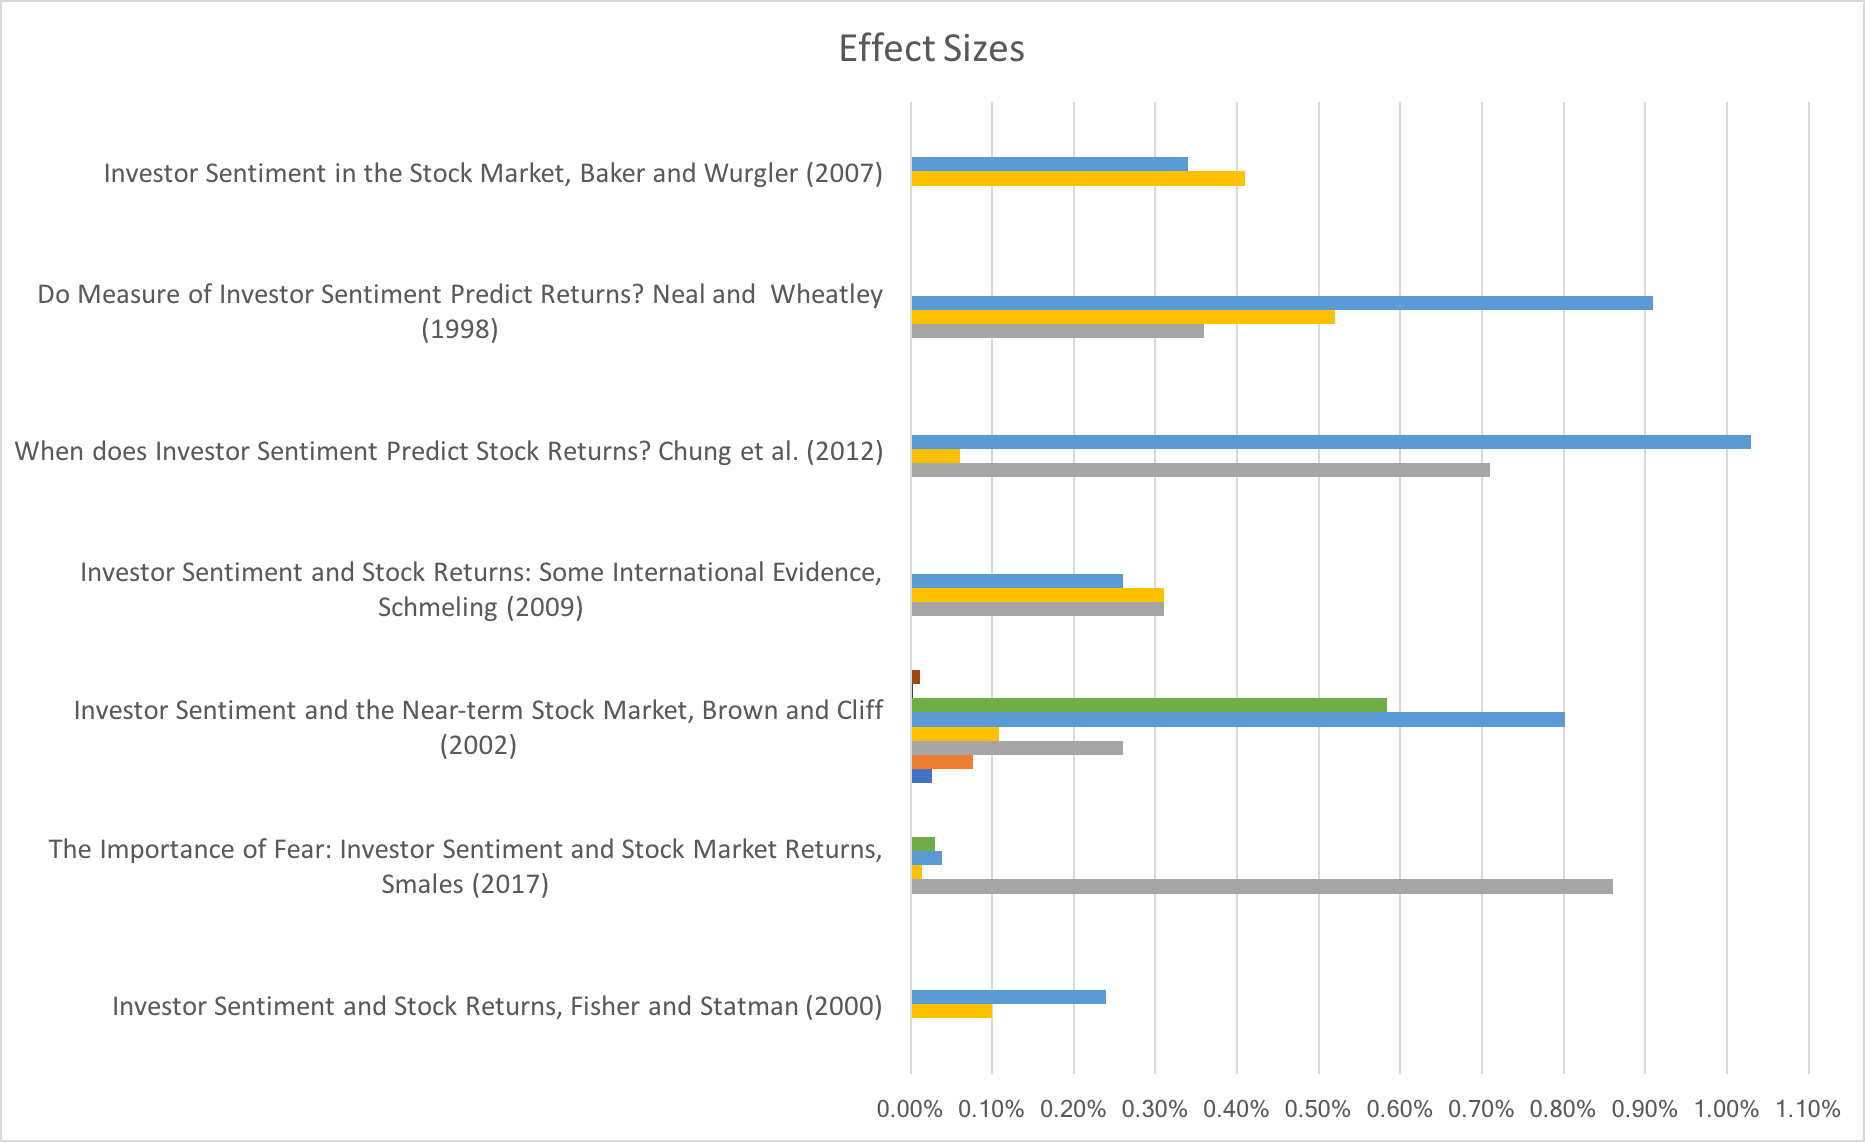
\includegraphics[width=1\textwidth]{figures/effect-size.png}
\caption{\label{fig:figure20}Selected Range of Effect Sizes of Past Studies. In Baker and Wurgler (2007) and Neal \& Wheatley (1998) the effect size is the change in returns if sentiment is one standard deviation above normal. For the remaining studies the effect size is the percentage change in return after one percent change in sentiment.}
\end{figure}

The data of Figure~\ref{fig:figure20} includes results from a variety of time lags from 1 to 6 months, as well as different sentiment measures, such as AAII or VIX. The effect size itself is: the percentage change in return if sentiment deviates by one standard deviation from historical average for Baker and Wurgler (2007) and Neal and Wheatley (1998); or the percentage change in stock returns after one percent change in sentiment level for the remaining studies. All studies found that investor sentiment and stock returns are negatively related. To mirror this finding in Figure~\ref{fig:figure20}, we inverted some of the effect sizes to receive a concise overview focusing on the strength of the relationship. The inversion was necessary because some studies, particularly Smales (2017), use a fear indicator instead of positive sentiment. Remarkably, no effect size approaches 1\%, except one finding by Chung et al. (2012). The change in stock returns is almost always smaller than the change in sentiment. Apart from that, the range of effect sizes is widespread between 0\% and 0.9\%. Conclusively, while there is agreement on the existence of a negative relationship, the effect size varies widely. This is caused by different measurements, methodologies and markets and stocks researched applied by the researchers. 

\section{Research Project Proposal} \label{research-proposal-section}
\subsection{Motivation}
The studies evaluated in the previous section applied traditional ways of measuring investor sentiment. In the following we explain why and how modern measurements add value to investor sentiment research, and illustrate how we will apply them in our own research.
\par
Traditional investor sentiment measures such as AAII or II have provided direct insights on investor sentiment for multiple decades and most of the studies have employed these measures to investigate the connection between investor sentiment and stock returns. Furthermore, indirect sentiment measures, such as VIX, consumer confidence, market performance or a weighted measure proposed by Baker and Wurgler (2007), which combines multiple indirect proxies, have been used to better understand the relationship. With the rise of technology and the internet, new ways to measure investor sentiment have emerged which are utilized by traders all over the world. Those new measures capture investor sentiment in two distinct ways. First, a new way to measure investor sentiment on a large scale appeared with the rise of the platform StockTwits, which is a social media platform specifically geared towards stock traders. Users exchange thoughts on stocks and indices by posting messages and engaging in conversations. Hereby, they can specifically label their posts as bearish or bullish and thus directly share their sentiment. With 7 million monthly active users, StockTwits contains a large array of sentiment data and this sentiment is likely to have an impact on the decision making process of the individual investor. Collecting and organizing this data allows an entirely new, big-data based approach to measuring investor sentiment - similar to the surveys employed by organizations such as AAII or II on a large scale. The advantage of these new big data approaches over traditional methods is that for the first-time, sentiment towards specific stocks or indices can be related to the returns of that specific stock or index. The amount of data enables researchers to analyse sentiment and returns on a daily basis, not only weekly or monthly. Moreover, it is now possible to analyse whether the so-called "wisdom of the crowds" adds value to the stock market and to financial industry.
\par
The second approach to measuring sentiment is through intelligent algorithms which scan social media platforms for stock-related posts and employ Natural Language Processing (NLP) algorithms to categorize these tweets as bullish or bearish. The goal of successful NLP is to train computers to correctly process natural language and categorize text as a human brain would. Prior research on investor sentiment on Twitter and subsequent stock returns was conducted by Bollen et al. (2011), Rao et al. (2012), Chen et al. (2013) and Skuza et al. (2015). These authors developed own algorithms which classify whether the tweet about a certain stock is bullish, bearish or neutral. With computing power becoming cheaper and more readily available, organizations developed own NLP algorithms and are using them on large scale. PsychSignal is such an organization; their algorithms evaluate both the Twitter and the StockTwits feeds and translate each post into bullish or bearish sentiment. The characteristics of posts are then aggregated by the related symbol and day. PsychSignal offers all their data to the public for free on Quantopian, a platform where researchers can use this investor sentiment measure to experiment new connections between stock returns and investor sentiment. This data is also used by professional, quantitative investors to develop and improve their trading algorithms.
\par
The goal of our research is to evaluate these modern investor sentiment measures, which are used by the public and influence investment decisions. Our research approach is on three levels: (1) compare these new sentiment measures to more traditional measures like AAII (2) compare the PsychSignal NLP algorithm to the direct sentiment measure from StockTwits users and (3) investigate the relationship between the modern investor sentiment measures and stock returns, which is the main hypothesis of our research. 

\subsection{Research Strategy} \label{research_strategy}
For the first and second level of our research, we will apply time series studies, focusing on correlation analyses. There are three modern sentiment measures (databases) available to us which will be used in this research: (1) StockTwits (direct sentiment measure from StockTwits users), (2) PS:StockTwits (StockTwits messages analysed by the PsychSignal NLP algorithm) and (3) PS:Aggregated (aggregated Twitter and StockTwits messages analysed by the PsychSignal NLP algorithm). Since data mining and text sentiment analysis are two modern and new concepts, we are interested in investigating the extent to which the results of the modern way of capturing investor sentiment through social media and tweets overlaps with the traditional sources of investor sentiment employed in existing studies. Furthermore, we decided to investigate the relationship between different modern sentiment measures since they differ in the way data is collected. The correlation analysis is a viable tool in this situation since our interest is in correlation/association and not causation. A high correlation between the measures shows that the sentiment measures follow a similar pattern, whereas low correlation implies that the sentiment measures differ. This test will not imply causation.
\par
The research strategy for the third level of our research points to the main hypothesis effect of investor sentiment on subsequent stock returns. For this specific research question, the perfect strategy would be an experimental study. Experiments are the most powerful tool in proving direct causation since only the independent variable is manipulated, while other variables and factors are kept constant. On the one hand, this results in high internal validity of the strategy, ensuring we have found a direct effect of the independent variable on the dependent one. On the other hand, an experimental study applied to investor sentiment and stock returns comes with many barriers which cannot be overcome.
\par
There are two main problems with an experiment. Firstly, the limited time frame of this study makes it impossible to conduct an experiment which has generalizable results. The analysis of investor sentiment over stock returns should be conducted over a longer period so that a general trend can be observed, and not just temporary positive or negative trends. Since the time frame of our research has a timespan of few months, this period is not sufficient to draw precise conclusions. Secondly, an experiment suggests that the experimental groups should not be influenced by any external factors. Regarding investor sentiment, this implies that investors cannot be allowed to access information other than what is provided by the researchers. In this case, participants must be controlled and finding willing people to be part of this study might not be easily achieved.
\par
With experiments not being a feasible option, the research strategy which fits our purposes is the panel study. Although it presents lower internal validity for causal claims, it solves many of the dilemmas posed by the experiment, and, furthermore, it has a higher level of ecological validity: the findings can be generalised to the real-life since the researcher has little to no influence. The panel study is suitable in this case because we want to study how changes in the independent variable affect the dependent variable over time. Moreover, having two continuous variables and studying only two stocks (as explained in the next section), it is possible to employ a time series study, where the panel is made of the data points at a certain moment in time for only one focal unit. This time series study allows the use of time lags between variables. Our point of interest is the regression coefficient which is discussed in section \ref{effect size parameter} in more detail.

\subsection{Population} \label{population}
Regarding the population of interest, we plan to investigate the effect of investor sentiment on S\&P 500 and Dow Jones Industrial Average (DJIA) stocks. DJIA stocks are large, traditional American firms, whereas S\&P 500 has a wider breadth of companies from different industries, with different market capitalisation and volatility. Since there is not sufficient investor sentiment data for each individual stocks from S\&P 500 and DJIA, we decided to work with indices and not at an individual stock-level. Indices are useful in measuring the value of a given section of the market, and they also provide a reliable proxy for the performance of the containing stocks (Fisher and Statman 2000, Brown and Cliff 2006). Considering the availability of sentiment data in our data sources, the final decision was to use exchange-traded funds (ETFs) which specifically track S\&P 500 and DIJA. These index funds seek to replicate the performances of their respective indices. Hence, for S\&P 500 we use the S\&P 500 Index ETF, denoted \$SPY, and for the Dow Jones Industrial Average we employ the DJIA ETF, referred to as \$DIA.

\subsection{Time Frame} \label{timeframe}
The current literature varies in terms of time frame, aggregation of data and time lags. Because our research employs modern approaches of investor sentiment measures, these characteristics are mainly determined by the practical side of the research. The available data from StockTwits starts in 2010; however, since the platform's popularity grew over the years, the data from the first years is insufficient to draw conclusions for the overall investor sentiment regarding a certain stock or ETF. Similarly, PsychSignal provides different datasets which start in between 2009 and 2010 and also contain small numbers of analysed messages for the first years. Furthermore, the data we received was daily and many data points did not provide a reliable measure of investor sentiment for that day because of a lack of posts.
\par
Considering the above-mentioned reasons, we have aggregated the daily data regarding symbols \$SPY and \$DIA on weekly and monthly basis. Then, in order to decide on a time frame for our analysis, we have computed the means of these aggregated values to observe how the average number of weekly and monthly analysed posts have changed over the years. Figures~\ref{fig:msg_spy_agg} and~\ref{fig:msg_dia_agg} below present these values for sentiment data from the dataset PS:Aggregated over the period 2012-2016.

\begin{figure}[ht]
\centering
\caption{\label{fig:msg_spy_agg}Analysed posts by NLP algorithm for symbol \$SPY}
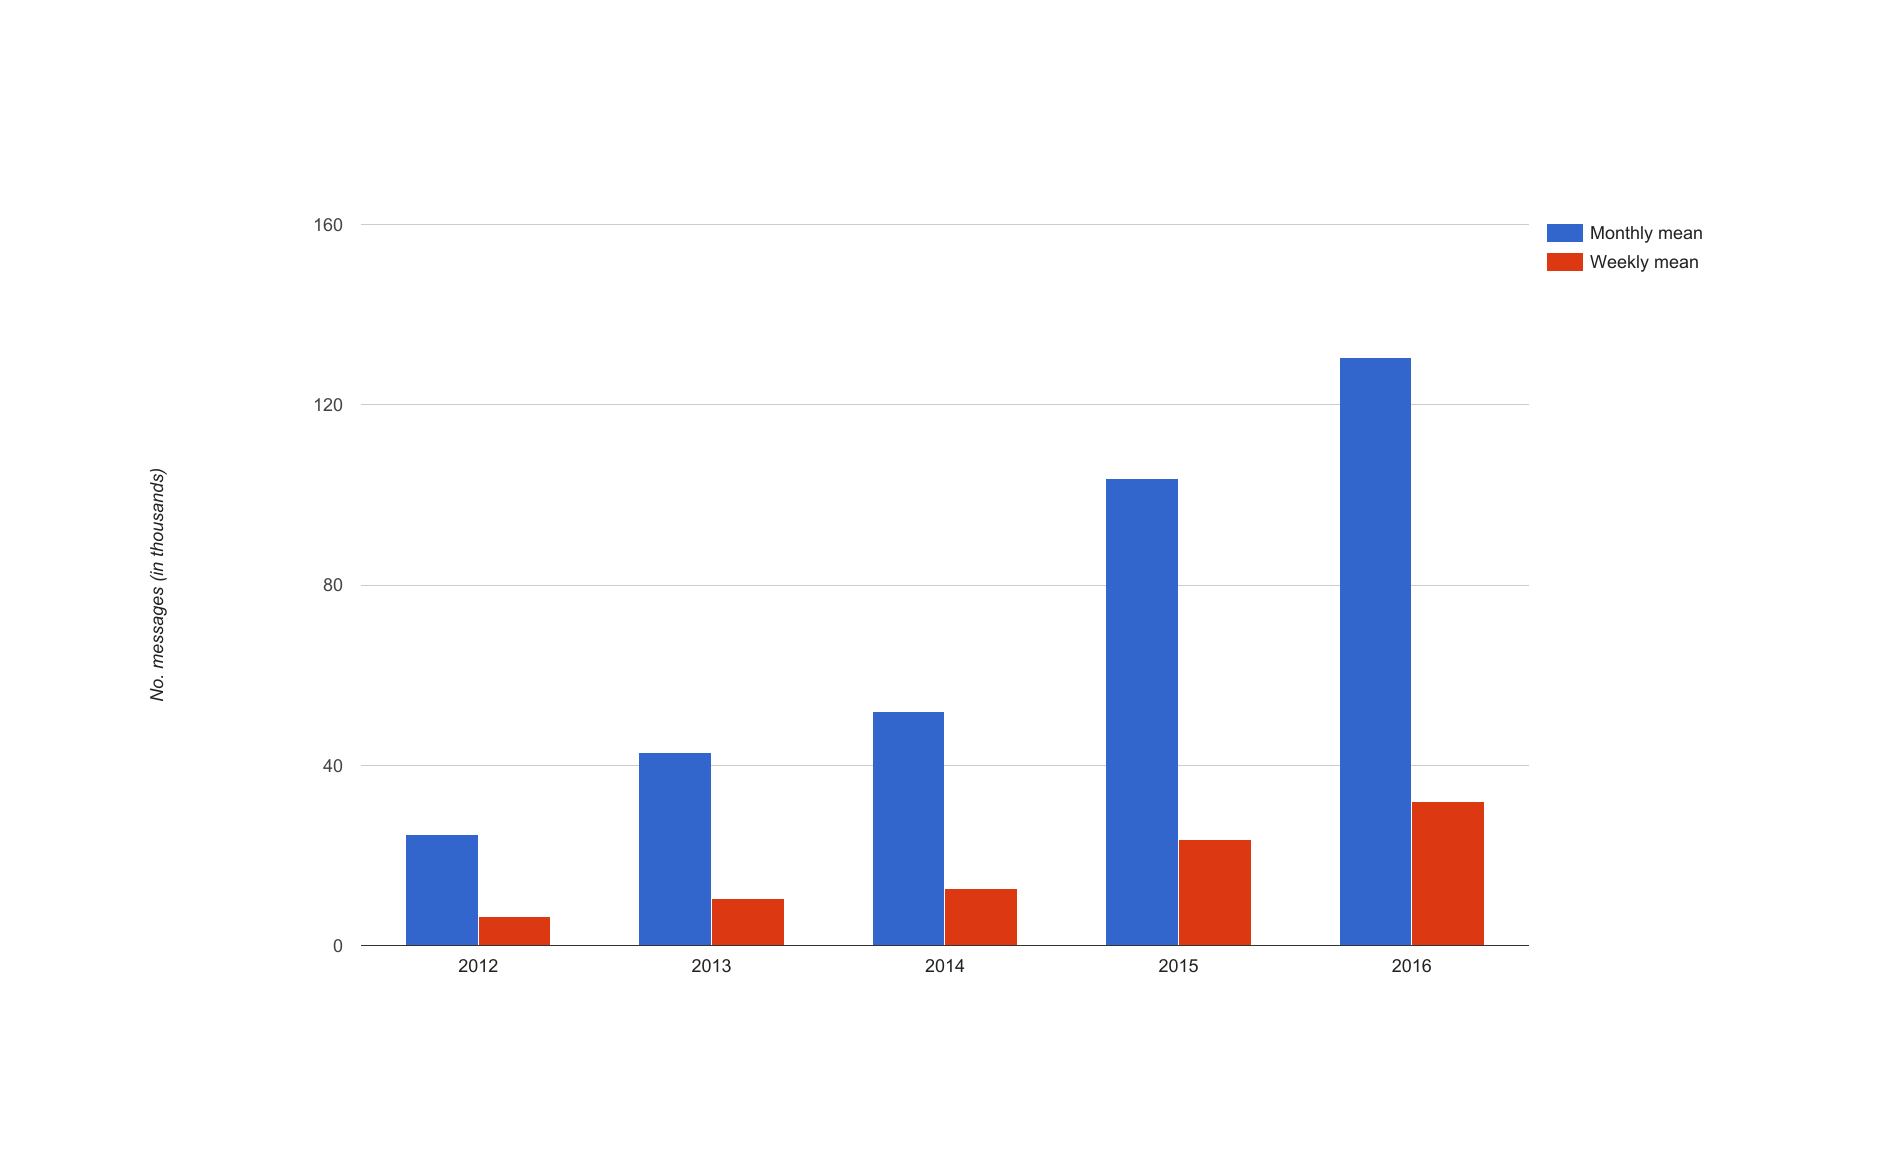
\includegraphics[width=0.8\textwidth]{figures/msg_spy_agg.png}
\end{figure}

\begin{figure}[ht]
\centering
\caption{\label{fig:msg_dia_agg}Analysed posts by NLP algorithm for symbol \$DIA}
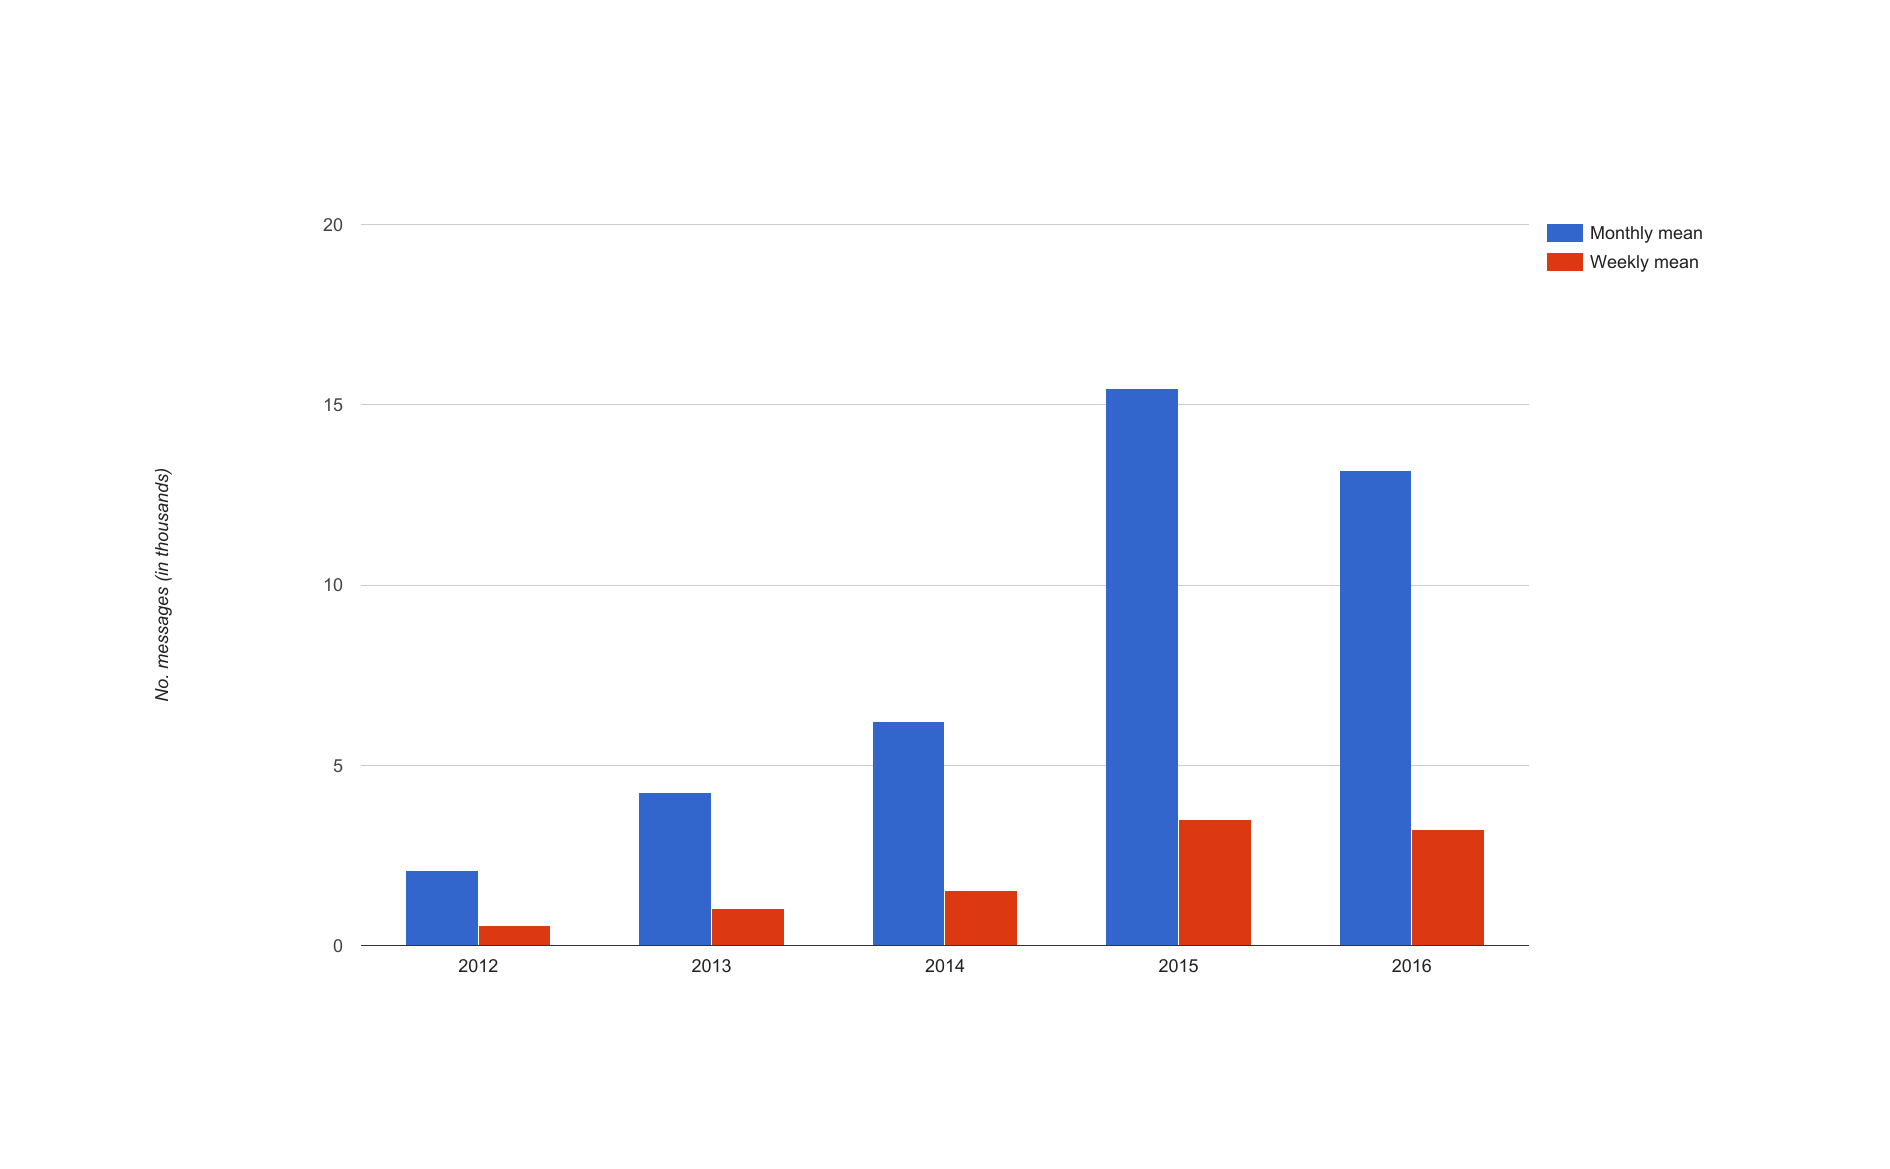
\includegraphics[width=0.8\textwidth]{figures/msg_dia_agg.png}
\end{figure}

The figures show a large difference between the years of interest. The monthly mean of \$SPY related posts increased from 24,531 in 2012 to 130,531 in 2016, while \$DIA related posts started at 2,094 in 2012 and reached 13,167 in 2016. The weekly means show similar trends, reaching five times the initial values. Based on these results, we have decided to work with data from 01/01/2014 until 31/12/2016, covering three full years.
\par
Regarding the time lags studied, we chose to pursue multiple time lags in order to investigate the effect of sentiment both on short-term and long-term returns. Hence, we choose weekly lags of 1, 4, 6, 8 and 12 weeks, and monthly lags of 1, 2 and 3 months.

\subsection{Data Matrix}
The choice of research strategy has a high impact on the data matrix and its structure. Since our research is time-series study (a type of panel study), the data matrix needs to present the changes in variables over time. The rows of the matrix represent different cases, and the columns are the characteristics of the case. Since the characteristics of the tests to be performed vary widely, we present a sample of the data matrix in Table~\ref{tab:data-matrix} below. This data matrix presents the ETF \$SPY, weekly aggregated data with 6-weeks lag, change in investor sentiment as independent variable and stock returns as dependent variable:

\begin{table}[ht]
\centering
\begin{tabular}{ c c c c }
Case (Stock: SPY) & Week & Change in investor sentiment & Stock return  \\\hline
SPY & 1 & \( \Delta sent_1 \) & \( return_7 \) \\
SPY & 2 & \( \Delta sent_2 \) & \( return_8 \) \\
SPY & 3 & \( \Delta sent_3 \) & \( return_9 \) \\
... & ... & \( ... \) & \( ... \) \\
SPY & 151 & \( \Delta sent_{151} \) & \( return_{157} \) \\
\end{tabular}
\caption{\label{tab:data-matrix}Example Data Matrix}
\end{table}

All the variations presented in sections~\ref{research_strategy},~\ref{population} and~\ref{timeframe} lead to 96 regression analyses which are different regarding the studied ETF, type of data aggregation, dataset, time lag and type of independent variable (absolute level of sentiment or change in level of sentiment). The regressions follow the formula below, where $\alpha$ is the intercept and $\beta$ is the regression coefficient:
\begin{equation}
Return_{t+lag} = \alpha + \beta * sentiment_t
\end{equation}

Plotting an exemplary time-series regression for \$SPY sentiment change, weekly aggregated, and returns six weeks later results in the graph presented in figure~\ref{fig:figure1}.

\begin{figure}
\centering
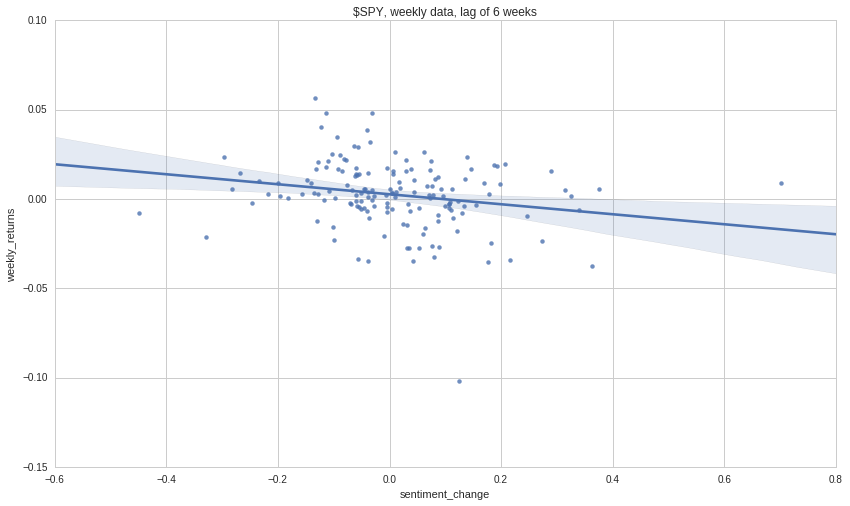
\includegraphics[width=1\textwidth]{figures/figure1.png}
\caption{\label{fig:figure1}Scatter Plot and Regression line}
\end{figure}

\newpage

\subsection{Measurement Protocol}
Although StockTwits and PsychSignal work with different algorithms and provide different ways to measure investor sentiment, the collection and manipulation of data leads to similar datasets. Data from StockTwits contains information about each post and the user who posted it, as well as data about the related stock; included in this is the indication whether the post is bullish, bearish or neutral. After storing this data in a database, we can filter it on the stocks of interest and make weekly or monthly aggregates on the number of bull and bear messages. The sentiment level is then determined as the percentage of bullish messages from the total of bullish and bearish messages:
\begin{equation}
BullPerc = Bull_{messages} / (Bull_{messages} + Bear_{messages})
\end{equation}
To compute the change in sentiment level in period t+1, we use the following formula:
\begin{equation}
Sent_{change} = (BullPerc_{t+1} - BullPerc_t ) / BullPerc_t
\end{equation}
For PsychSignal data, the total number of bullish and bearish messages is already aggregated daily, and thus we can use these totals. After filtering the data on stock and date, we sum up the numbers on weeks or months, according to our time-frame. The percentage of bullish messages per period and the change in it are computed using the same formulas as above.

\subsection{Specification of the Effect Size Parameter} \label{effect size parameter}
After establishing the cases in the above data matrix using the data from StockTwits, PsychSignal and stock return data, we will quantify the strength of the relationship by establishing an effect size. For the comparison of different measures of investor sentiment, the correlation coefficient is used. With this coefficient, we measure whether there is linear relationship between two variables and the strength and direction of this relationship. The coefficient of correlation takes values between -1 and 1, where r=1 shows a very strong positive relationship. 
\par
To measure the magnitude of the relationship between investor sentiment and stock returns, we use regression coefficients. We test with both the change and the absolute value of investor sentiment as independent variable. When change in sentiment is used, the effect size denotes the magnitude of the stock return change influenced by the change in investor sentiment. When using absolute values, we investigate what is the magnitude of the influence of level of sentiment on stock returns.

\section{Results} \label{results-section}
Having established our research design, this section presents the results of the analyses conducted. First, we describe the stock returns and investor sentiment data, while also looking at the types of companies found in S\&P 500 and DJIA, and the types of investors using the platform StockTwits. Then, we study the relationship between trading volume and number of sentiment messages, and the correlations between different investor sentiment measures, both traditional and modern. This allows us to better understand when users express their sentiment and whether this behaviour is influenced by higher volatility. Finally, the results of the third level of our research are presented, where we test what is the relationship between modern investor sentiment measures and subsequent stock returns.

\subsection{Descriptive Statistics}
Descriptive statistics present information about the data used and summarises its important features. In the quantitative analysis, we are most interested in the mean, the standard deviation and the number of observations of the dataset in order to have an indication of data variability. These features are presented in the following subsections.

\subsubsection{Dependent Variable: Stock Returns}
Table~\ref{tab:table4} below summarizes the monthly and weekly returns of \$SPY and \$DIA for the period 01/01/2014 - 31/12/2016. The means of returns are slightly positive and almost identical for both ETFs. Surprisingly, \$DIA has higher standard deviation both on a monthly and weekly basis, even though it mostly consists of large companies. S\&P500 presents a more diversified portfolio which in turn might reduce the variability between returns. An interesting contrast is the existence of more extreme minimum and maximum values for \$DIA compared to \$SPY.


\sbox\tempbox{%
\begin{tabular}{@{}lllll@{}}
\toprule
        & \multicolumn{2}{l}{\textbf{Monthly}} & \multicolumn{2}{l}{\textbf{Weekly}} \\ \midrule
        & \$SPY             & \$DIA            & \$SPY            & \$DIA            \\
Mean    & 0.0087            & 0.0086           & 0.0016           & 0.0015           \\
Std Dev & 0.0324            & 0.0339           & 0.0190           & 0.0192           \\
Min     & -0.0737           & -0.0765          & -0.1017          & -0.1024          \\
Max     & 0.0884            & 0.0903           & 0.0566           & 0.0606           \\
N       & 36                & 36               & 157              & 157              \\ \bottomrule
\end{tabular}%
}
\setlength\templen{\wd\tempbox}
\begin{table}[h]
\centering
\usebox{\tempbox}\\[3pt]
\parbox{\the\templen}{\small This table shows descriptive statistics for the weekly and monthly returns of \$SPY and \$DIA ETFs.}
\caption{Descriptive Statistics of Stock Returns}
\label{tab:table4}
\end{table}


\subsubsection{Description of Companies in S\&P 500 and DJIA}
Dow Jones Industrial Average consists of 30 companies, which are large, traditional American corporations with long history. The companies in S\&P500 are picked by the S\&P committee and are generally the 500 largest publicly traded companies on the US market. Therefore, S\&P 500 is more diverse and includes also companies with lower market capitalization. Figures~\ref{fig:figure2} and~\ref{fig:figure3} below show both indices divided by industry.

\begin{figure}[ht]
\centering
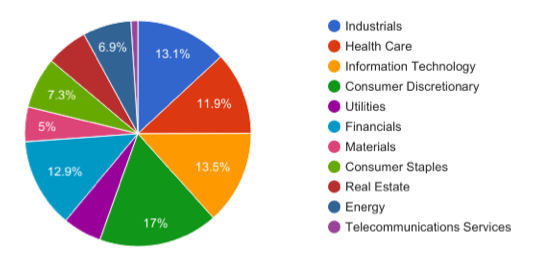
\includegraphics[width=0.75\textwidth]{figures/figure2.png}
\caption{\label{fig:figure2}Industries of Companies in S\&P 500}
\end{figure}

\begin{figure}[ht]
\centering
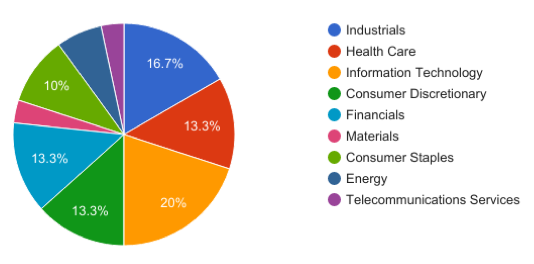
\includegraphics[width=0.75\textwidth]{figures/figure3.png}
\caption{\label{fig:figure3}Industries of Companies in DJIA}
\end{figure}

The graphs visualize that both S\&P 500 and DJIA have a wide spread of companies from all major industries. Our research is therefore not limited to a specific branch but allows generalization to different industries on the US market.

\newpage

\subsubsection{Independent Variable: Investor Sentiment}
As mentioned before in section~\ref{research_strategy}, we gather investor sentiment data from three data sources, which are statistically described in this section.
\par
Table~\ref{tab:spy-descriptives} below summarizes the descriptive statistics of investor sentiment measures for \$SPY. The sentiment level is defined as the percentage of bullish posts; therefore, it is in the interval [0,1].

\sbox\tempbox{%
  \begin{tabular}{crrrrrrr}
    \multicolumn{2}{c}{\textbf{\$SPY}} & \multicolumn{3}{c}{\textbf{Monthly}} & \multicolumn{3}{c}{\textbf{Weekly}} \\
    \toprule
    \multicolumn{2}{c}{Source} & \multicolumn{2}{c}{PsychSignal} & \multicolumn{1}{c}{StockTwits} & \multicolumn{2}{c}{PsychSignal} & \multicolumn{1}{c}{StockTwits} \\
    \midrule
    \multicolumn{2}{c}{Database} & \multicolumn{1}{c}{\specialcell{PS:\\ Agg.}} & \multicolumn{1}{c}{\specialcell{PS: \\StockTwits}} & \multicolumn{1}{c}{StockTwits} & \multicolumn{1}{c}{\specialcell{PS: \\Agg.}} & \multicolumn{1}{c}{\specialcell{PS: \\StockTwits}} & \multicolumn{1}{c}{StockTwits} \\
    \midrule
    \multirow{5}[0]{*} {\specialcell{Absolute \\ Sentiment}}
     & Mean  & 0.5991 & 0.5948 & 0.4181 & 0.6009 & 0.5962 & 0.4184 \\
          & Std dev & 0.0464 & 0.0197 & 0.0623 & 0.0637 & 0.0330 & 0.0922 \\
          & Min   & 0.4944 & 0.0541 & 0.2701 & 0.3660 & 0.5210 & 0.2161 \\
          & Max   & 0.7535 & 0.6334 & 0.5199 & 0.8198 & 0.6905 & 0.6540 \\
          & N     & 3613956 & 1418685 & 204547 & 3613956 & 1418685 & 204547 \\
    \multirow{5}[0]{*} {\specialcell{Change in \\ Sentiment}} & Mean  & 0.0066 & 0.0026 & 0.0157 & 0.0102 & 0.0025 & 0.4518 \\
          & Std dev & 0.0949 & 0.0412 & 0.1781 & 0.1449 & 0.0691 & 0.1695 \\
          & Min   & -0.0204 & -0.0636 & -0.2523 & -0.4484 & -0.2290 & 0.0667 \\
          & Max   & 0.2610 & 0.0851 & 0.5465 & 0.7017 & 0.1692 & 10,000 \\
          & N     & 3613956 & 1418685 & 204547 & 3613956 & 1418685 & 204547 \\
          
          \bottomrule
    \end{tabular}%
}
\setlength\templen{\wd\tempbox}
\begin{table}[htbp]
\centering
\usebox{\tempbox}\\[3pt]
\parbox{\the\templen}{\small This table shows the descriptive statistics of investor sentiment data of ETF \$SPY for the studied period. Sentiment data is aggregated both on weeks and months, and the table includes the description of all three datasets.}
\caption{Descriptive statistics for investor sentiment of \$SPY}%
\label{tab:spy-descriptives}%
\end{table}%


For both investor sentiment measures provided by PsychSignal we were able to collect large amounts of data points, precisely between 1.5 million and 3.6 million. Messages with sentiment label on StockTwits, thereby being categorised as direct measurement, were approximately 200,000. The means of the bullish percentages of \$SPY posts from both PS:Aggregated and PS:StockTwits are very similar, close to 60\%. Monthly values stay close to the mean, whereas the minimum and maximum values of the weekly sentiment have a larger spread. The minimum sentiment measure from PS:Aggregated of \$SPY is 36.6\%, while the maximum is 81,98\%.
\par
Looking for differences between direct sentiment measure on StockTwits and the data provided by PsychSignal, the first major noticeable difference is the large difference between the means of bullish percentage. The bullish percentage from StockTwits is only about 41.81\% (both for months and weeks), compared to the 60\% from PS:StockTwits. As a result, we can conclude that users are more likely to provide bearish labels with their messages or the NLP algorithm is skewed towards positivity. Moreover, this also implies that unlabelled messages can be evaluated often as bullish by PsychSignal's NLP. Which measure shows the strongest relationship to subsequent stock returns will be discussed in section~\ref{sentiment-measure-discussion}. The correlation between the measurements obtained from PsychSignal and StockTwits are analysed in section~\ref{correlation-sentiments}. Table~\ref{tab:dia-descriptives} below summarizes the descriptive statistics on investor sentiment measures for \$DIA.

\sbox\tempbox{%
    \begin{tabular}{crrrrrrr}
    \multicolumn{2}{c}{\textbf{\$DIA}} & \multicolumn{3}{c}{\textbf{Monthly}} & \multicolumn{3}{c}{\textbf{Weekly}} \\
    \toprule
    \multicolumn{2}{c}{Source} & \multicolumn{2}{c}{PsychSignal} & \multicolumn{1}{c}{StockTwits} & \multicolumn{2}{c}{PsychSignal} & \multicolumn{1}{c}{StockTwits} \\
    \midrule
 	\multicolumn{2}{c}{Database} & \multicolumn{1}{c}{\specialcell{PS: \\Agg.}} & \multicolumn{1}{c}{\specialcell{PS: \\StockTwits}} & \multicolumn{1}{c}{StockTwits} & \multicolumn{1}{c}{\specialcell{PS: \\Agg.}} & \multicolumn{1}{c}{\specialcell{PS: \\StockTwits}} & \multicolumn{1}{c}{StockTwits} \\
    \midrule
    \multirow{5}[1]{*}{\specialcell{Absolute \\sentiment}} & Mean  & 0.6012 & 0.6096 & 0.4377 & 0.6194 & 0.6124 & 0.4518 \\
          & Std dev & 0.1273 & 0.0531 & 0.1003 & 0.1516 & 0.0802 & 0.1695 \\
          & Min   & 0.2824 & 0.4943 & 0.2793 & 0.1603 & 0.4268 & 0.0667 \\
          & Max   & 0.7474 & 0.7233 & 0.6932 & 0.8765 & 0.8718 & 1000 \\
          & N     & 437618 & 65747 & 5542  & 437618 & 65747 & 5542 \\
    \multirow{5}[0]{*}{\specialcell{Change in \\sentiment}} & Mean  & 0.0701 & 0.0080 & 0.0322 & 0.0881 & 0.0131 & 0.1638 \\
          & Std dev & 0.4167 & 0.1246 & 0.3009 & 0.5322 & 0.1690 & 0.7603 \\
          & Min   & -0.5099 & -0.1923 & -0.3710 & -0.6935 & -0.3615 & -0.7537 \\
          & Max   & 13977 & 0.3306 & 0.7279 & 30471 & 0.5378 & 52,473 \\
          & N     & 437618 & 65747 & 5542  & 437618 & 65747 & 5542 \\
          \bottomrule
    \end{tabular}%
}
\setlength\templen{\wd\tempbox}
\begin{table}[htbp]
\centering
\usebox{\tempbox}\\[3pt]
\parbox{\the\templen}{\small This table shows the descriptive statistics of investor sentiment data of ETF \$DIA for the studied period. Sentiment data is aggregated both on weeks and months, and the table includes description of all three datasets.}
\caption{Descriptive statistics for investor sentiment of \$DIA}
\label{tab:dia-descriptives}%
\end{table}%



\par
The numbers follow a similar pattern as described for ETF \$SPY. There is less activity for \$DIA on social media than for \$SPY, resulting in fewer data points available. However, with a minimum of 30 messages per week there is enough data available to draw conclusions about the investor sentiment. The most striking difference between both PsychSignal data sources and StockTwits is again a lower bullish percentage if users directly state their sentiment. Therefore, lower sentiment when explicitly asked seems to generally apply for most stocks/indexes.

\subsubsection{Type of investors on investment platform StockTwits}
StockTwits allows users to define their Experience, Investing Approach and Holding Period. Below are the distribution graphs of StockTwits users based on these three variables. StockTwits users have mainly intermediate experience, with focus on short term investments and growth, technical and momentum strategies.
\par
While we do not differentiate in our research between investor groups, the information about the distribution carries value because it shows which types of investors leave their opinions on social media. The distributions for each investor distinction are even. The investing approaches from traders range from growth to value (Figure ~\ref{fig:figure4}), with most traders applying a technical approach. This is not surprising, since PsychSignal and StockTwits is used by traders who are interested in maximizing their returns by applying quantitative strategies and algorithms. 

\begin{figure}[ht]
\centering
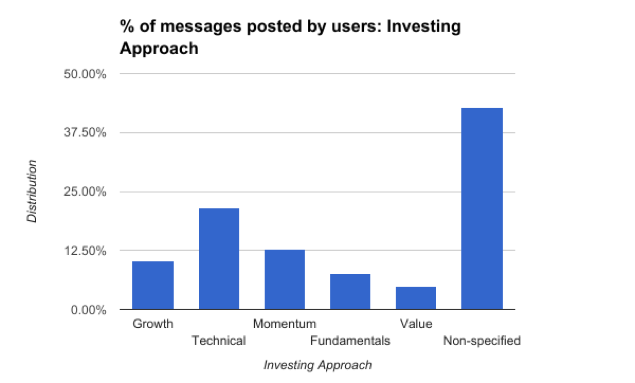
\includegraphics[width=0.6\textwidth]{figures/figure4.png}
\caption{\label{fig:figure4}Investing Approach}
\end{figure}

The traders' experience as classified by themselves is mostly intermediate (30\%), and the novices and professional investors have almost equal proportions (each approximately 15\%). Therefore, our research cannot be categorized by investor types, but is more an indicator of sentiment across all trader groups.

\begin{figure}[ht]
\centering
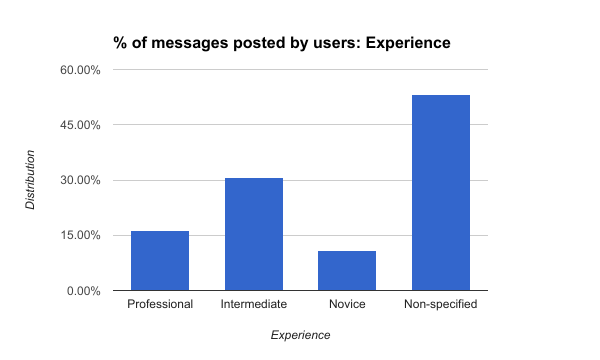
\includegraphics[width=0.6\textwidth]{figures/figure5.png}
\caption{\label{fig:figure5}Trader Experience}
\end{figure}

Lastly, we looked at the holding period of the traders posting messages on StockTwits. Once more, traders apply a range of different methods, from swing traders to long-term investors. 

\begin{figure}[ht]
\centering
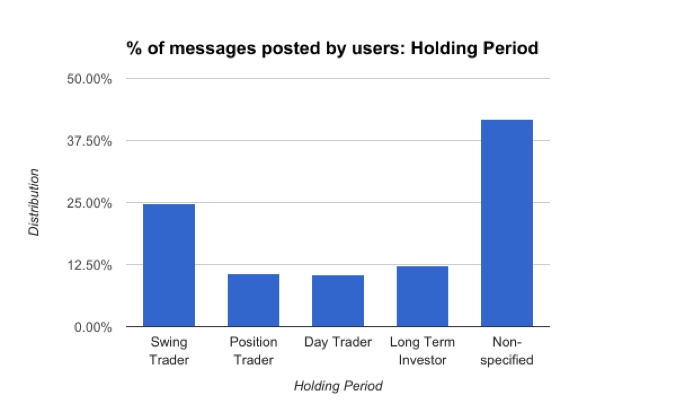
\includegraphics[width=0.6\textwidth]{figures/figure6.png}
\caption{\label{fig:figure6}Holding Period}
\end{figure}

Conclusively, our results will indicate relationships for aggregates of different investor types and investment approaches. To conduct research that evaluates the relationship between stock-specific sentiment and returns of that stock and also differentiate between investor groups, more data points are required. Separating by investor groups would cause the amount of data points available per week to fall significantly. 

\subsection{Relationship between Trading Volume and number of sentiment messages}
In previous researches of social media investor sentiment and sentiment derived via NLP algorithms and its relationship to stock returns (Bollen et al. 2011, Rao et al. 2012, Chen et al. 2013 or Skuza et al. 2015), the authors outlined that increased trading volume is positively correlated with increased number of sentiment messages. We run the tests for both \$SPY and \$DIA and StockTwits messages to see whether this holds true in our data. The correlation scatter plots 
are Figure~\ref{fig:figure7} and Figure~\ref{fig:figure8} respectively.

As expected we can see a strong positive relationship between the trading volume and the number of StockTwits messages for \$SPY and \$DIA. This notion highlights that when a financial instrument is traded in abnormal volumes, people tend to share more sentiment and more opinions about its development. This shows that the investor's react strongly towards high trading volumes (usually after an important event occurs) and share sentiment. It implies that the sentiment measured is strongly influenced by recent events and might not reflect primarily the opinion of investors based on thorough analysis in the long term. This contrasts with the way how AAII measures investor sentiment, where the investors share their opinion about the market in 6-month lag. These results seem to be consistent with the nature of individual investors, especially those, who focus on shorter-term trades using growth, technical or momentum strategies. Figure~\ref{fig:figure6} shows that these types of investors are prevalent on StockTwits. Thus, we expect that investor sentiment measured by StockTwits will be influencing stock returns in near term.

\newpage

\begin{figure}[h]
\centering
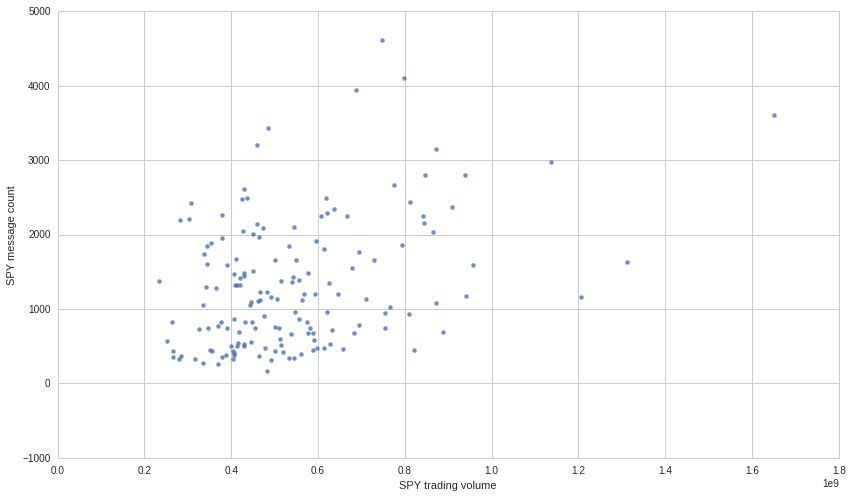
\includegraphics[width=0.8\textwidth]{figures/figure7.png}
\caption{\label{fig:figure7}Correlation Trading Volume and posts about \$SPY. p-value = 0.0000; coefficient =  0.3747 }
\end{figure}

\begin{figure}[h]
\centering
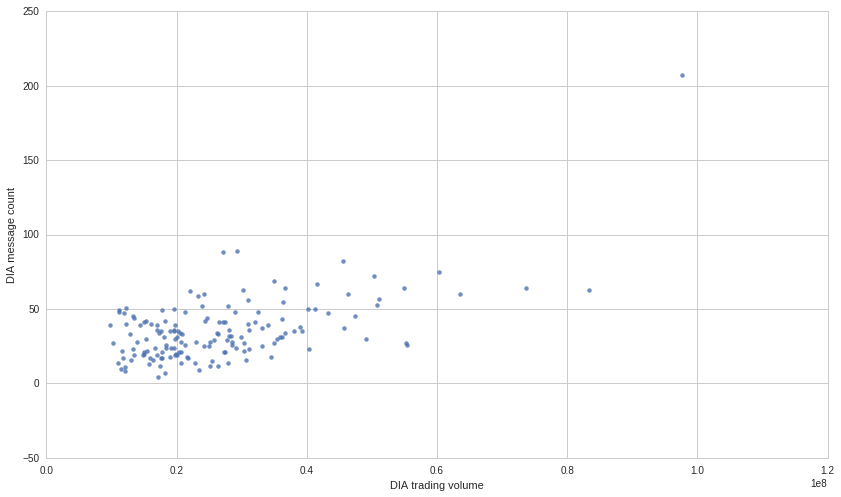
\includegraphics[width=0.8\textwidth]{figures/figure8.png}
\caption{\label{fig:figure8}Correlation Trading Volume and posts about \$DIA. p-value = 0.0000; coefficient = 0.5927}
\end{figure}

\newpage

\subsection{Correlation analyses between investor sentiment measures} \label{correlation-sentiments}
In this section, we look at levels 1 and 2 of our research, where we compare the modern sentiment measures with the traditional sentiment survey employed by AAII. Furthermore, we analyse the degree of association between different modern sentiment measures.

\subsubsection{Modern sentiment measures}
As seen in the descriptive statistics, there exist differences in the investor sentiment measures that we employ in our research. We compare \$SPY and \$DIA sentiments from the three databases both on weekly and monthly basis. All pairs investigated, except for two instances, exhibit relationship at the 1\% significance level with a coefficient of correlation between 0.21 and 0.72. The table with all the results can be found in Appendix, Table~\ref{tab:appendix2}.
\par
The highest coefficient is between monthly \$SPY from PS:StockTwits and monthly \$DIA from PS:StockTwits. Interestingly, the same pair, but with direct sentiment measure from StockTwits is not significantly correlated. This result follows the notion from descriptive statistics: the standard deviation of StockTwits measure is higher than PS:StockTwits.
\par
For \$SPY sentiment, StockTwits PS:StockTwits and StockTwits correlate at 1\% confidence level (0.55). For \$DIA, this relationship is similar, with coefficient of 0.57 at 1\% level.

\subsubsection{AAII and StockTwits direct investor sentiment measure}
To check how the contemporary investor sentiment measures compare to the more traditional ones, we analysed the connection between AAII and direct StockTwits sentiment measure through a correlation analysis.

\begin{figure}[ht]
\centering
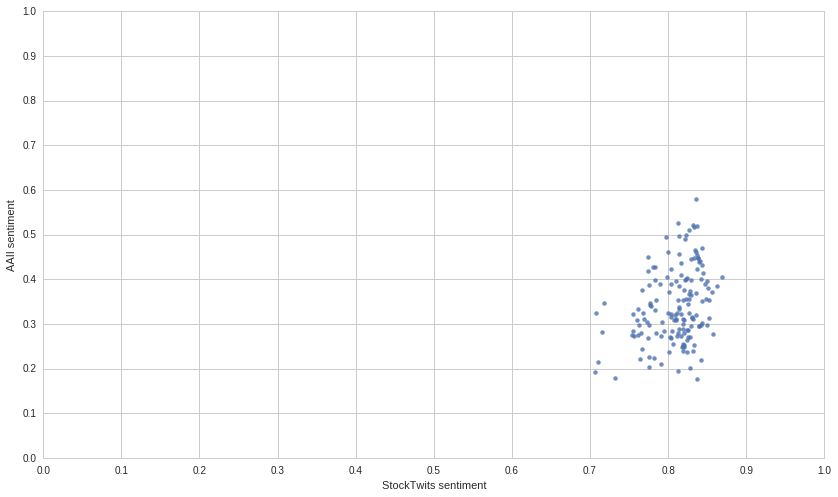
\includegraphics[width=1\textwidth]{figures/corrST-AAII.png}
\caption{\label{fig:figure9}Correlation StockTwits and AAII ($r=0.3119$)}
\end{figure}

The relationship is significant (p-value < 0.000) with a correlation coefficient of 0.3119. This shows an existent, but weak-moderate correlation between these two sentiment measures. In comparison, according to Brown and Cliff (2004), AAII and Investor Intelligence correlate significantly with a coefficient of 0.47. We can conclude that the new, social media and big data approach correlates with traditional investment sentiment measures via surveys only moderately. One more thing which becomes clear from correlation analysis is the much stronger average bullishness sentiment on StockTwits as compared to the AAII surveys. One of the next steps is to analyse whether one of the measurement types carries more value in predicting future stock performance, discussed in section~\ref{discussion-section}.

\subsubsection{AAII and PsychSignal indirect investor sentiment measures}
Following the analysis of investor sentiment between two direct measures (AAII and StockTwits), we want to investigate how the modern indirect measures from PsychSignal correlate with the traditional AAII direct measure. Since AAII sentiment survey is a market-wide sentiment measure, the indirect measures employed from PsychSignal need to reflect a market-wide sentiment as well. For this reason, the datasets used have included all available sentiment data points.
\par
First, we run correlation test between PS:StockTwits and AAII, which shows highly significant results with p-value ${\approx}$ 0.000, and a coefficient of correlation of 0.3963. This coefficient implies a weak-moderate positive relationship between the two sentiment measures and shows that PS:StockTwits dataset correlates with AAII to some extent. Figure~\ref{fig:figure10} shows the scatter plot for this relation between variables.

\begin{figure}[ht]
\centering
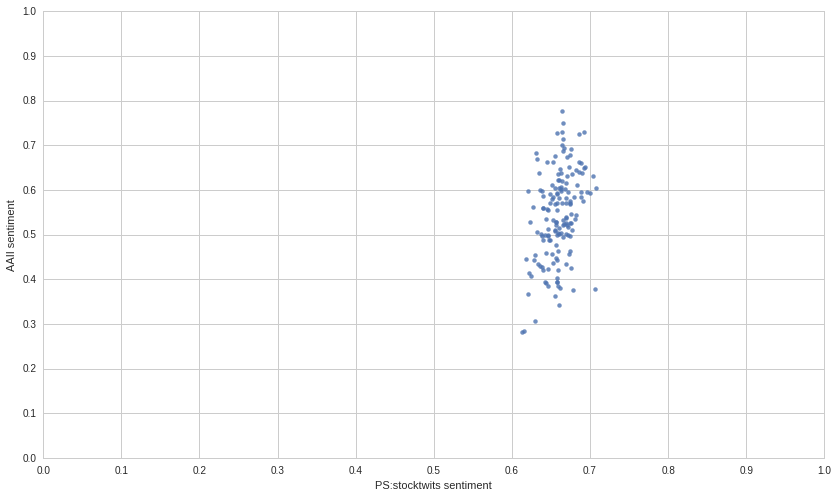
\includegraphics[width=1\textwidth]{figures/figure10.png}
\caption{\label{fig:figure10}Correlation PS:StockTwits and AAII (\textit{r}=0.3963)}
\end{figure}

The second correlation test is made between PS:Aggregated and AAII. Although the results are significant at the 10\% level (p-value = 0.0867), the Pearson correlation coefficient equals only 0.1372, indicating that there is a very weak association. This weak relationship can be observed in figure~\ref{fig:figure11}.

\begin{figure}[ht]
\centering
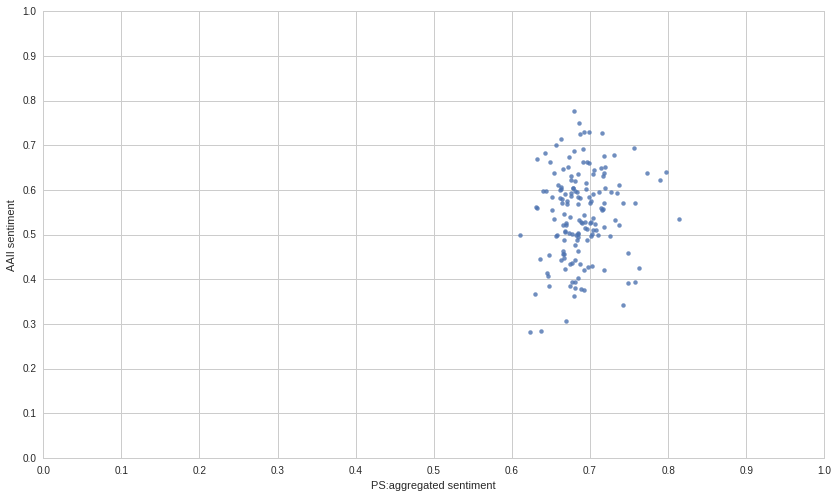
\includegraphics[width=1\textwidth]{figures/figure11.png}
\caption{\label{fig:figure11}Correlation PS:Aggregated and AAII (\textit{r}=0.1372)}
\end{figure}

A comparison of the two scatter plots clearly shows the difference between correlation coefficients. One of the explanations for this variation in results is given by the fact that dataset PS:Aggregated provides the results of an analysis of more messages than PS:StockTwits does, since the former includes Twitter posts in the analysis. This difference might reduce the overall bullishness feature or enhance the bearishness of sentiment. The previous results provide the basis of another correlation analysis between the market-wide sentiment measure given by the two PsychSignal datasets. Thus, running correlation analysis between PS:Aggregated and PS:StockTwits, the results are significant, with Pearson coefficient of 0.4627. Hence, this moderate relationship shows that these two datasets provide dissimilar sentiment measures.

\subsection{The relationship between modern investor sentiment measures and subsequent stock returns}

With significant correlations present between traditional and modern investor sentiment measures, we turn our attention to research level 3, which investigates the main hypothesis of the paper. In this part, we want to test whether periods with higher levels of investor sentiment are followed by periods with negative stock returns and vice versa. To investigate this relationship, we analyse the connection between subsequent stock returns and the three investor sentiment measures databases mentioned before: (1) StockTwits, (2) PS:StockTwits and (3) PS:Aggregated.
\par
We run univariate regressions which differ in lag, monthly or weekly periods and absolute value or the change in sentiment as the independent variable. All these factors have been highlighted in previous research as variables which produce different results. Since the research in the modern sentiment measures is new, our main goal is to establish basic relationships and thus we test for all these factors. The most significant outcomes are highlighted below, while all regression analyses results can be found in Appendix, Table~\ref{tab:appendix}.

\subsubsection{StockTwits - StockTwits direct sentiment measure}

\begin{center}

\itshape{
$H_{1a}:$ Investor Sentiment measured directly on StockTwits does not affect subsequent stock returns in S\&P 500.


$H_{1b}:$ Investor Sentiment measured directly on StockTwits does not affect subsequent stock returns in DJIA.
}

\end{center}

Both \$DIA and \$SPY have a significant (at 5\%) negative relationship between absolute StockTwits direct sentiment measured on weekly basis with 1 week lag. The effect sizes are -0.0198 and -0.0328, respectively. This means that 1\% increase in the sentiment measure leads to decrease of 0.00198 pp in \$DIA stock return. \$SPY exhibits a significant (5\%) result for the monthly period with 1 month lag. 
\par
Measuring the change of sentiment did not yield any significant results, except for \$DIA monthly with 3-month lag (10\% confidence level; effect size: 0.032). This relationship is positive, in contrast to previous results. Results indicate that the monthly change in sentiment is positively related to increase in returns on a longer term (3 months).

% Table generated by Excel2LaTeX from sheet 'stocktwits direct'
\sbox\tempbox{%
  \begin{tabular}{lccccrrr}
  & Type  & Agg.  & Database & Lag   & \multicolumn{1}{c}{Slope} & \multicolumn{1}{c}{p-value} & \multicolumn{1}{c}{$R^2$} \\
  \toprule
  \rowcolor[rgb]{ .949,  .949,  .949} \$SPY & Absolute & Weekly & StockTwits & 1-week & -0.0328** & 0.0367 & 2.80\% \\
  \rowcolor[rgb]{ .949,  .949,  .949} \$SPY & Absolute & Weekly & StockTwits & 6-week & -0.0253 & 0.1069 & 2.80\% \\
  \$DIA & Absolute & Weekly & StockTwits & 1-week & -0.0199** & 0.0283 & 3.08\% \\
  \rowcolor[rgb]{ .949,  .949,  .949} \$SPY & Absolute & Monthly & StockTwits & 1-month & -0.1531** & 0.0479 & 11.02\% \\
  \$DIA & Change & Monthly & StockTwits & 3-month & 0.0320* & 0.0612 & 10.22\% \\
  \bottomrule
  \end{tabular}%
}
\setlength\templen{\wd\tempbox}
\begin{table}[htbp]
\centering
\usebox{\tempbox}\\[3pt]
\parbox{\the\templen}{\small This table presents the results of the regression analysis between investor sentiment from StockTwits dataset and stock returns of \$SPY and \$DIA, aggregated weekly and monthly with different time lags. The asterisks mark the level of significance: ***: 0.01, **: 0.05, *: 0.10}
\caption{Results Regression of StockTwits direct sentiment and Stock Returns}
\label{tab:stocktwits-direct}%
\end{table}%


\subsubsection{PS: StockTwits - StockTwits indirect sentiment measure determined by PsychSignal}

\begin{center}

\itshape{
$H_{2a}:$ Investor Sentiment measured indirectly on StockTwits does not affect subsequent stock returns in S\&P 500.

$H_{2b}:$ Investor Sentiment measured directly by StockTwits does not affect subsequent stock returns in DJIA.
}

\end{center}

In contrast with the previous findings, absolute weekly \$SPY sentiment is not negatively related with 1 week lag in stock returns. \$DIA stays significant (10\%) on this level and the effect size increases to -0.0339.
\par
On the one hand, \$DIA weekly is significant for change in sentiment,both for 4 and 8 period lags. On the other hand, \$SPY is significant for change in sentiment in monthly periods with lag 2. For absolute values, 3-month lag is significant again with positive effect size. Also, other results, even not significant show positive slopes for the 3-month lag – the longest term what we analysed.
\par
The other significant results, \$DIA for 4 and 8-week lags, also exhibit positive relationships. Both are, as well, more long term. In contrast, \$SPY 2-month lag shows a negative relationship at 5\% level with a coefficient -0.2744.

% Table generated by Excel2LaTeX from sheet 'stocktwits indirect'
\sbox\tempbox{%
    \begin{tabular}{lccccrrr}
          & Type  & Agg.  & Database & Lag   & \multicolumn{1}{c}{Slope} & \multicolumn{1}{c}{p-value} & \multicolumn{1}{c}{$R^2$} \\
    \toprule
    \rowcolor[rgb]{ .949,  .949,  .949} \$SPY & Absolute & Weekly & PS: StockTwits & 1-week & -0.0543 & 0.2395 & 0.89\% \\
    \$DIA & Absolute & Weekly & PS: StockTwits & 1-week & -0.0339* & 0.0747 & 2.03\% \\
    \rowcolor[rgb]{ .949,  .949,  .949} \$SPY & Absolute & Monthly & PS: StockTwits & 3-month & 0.0487* & 0.0661 & 9.59\% \\
    \rowcolor[rgb]{ .949,  .949,  .949} \$SPY & Change & Monthly & PS: StockTwits & 2-month & -0.2744** & 0.0335 & 12.98\% \\
    \$DIA & Change & Weekly & PS: StockTwits & 4-week & 0.0146* & 0.0970 & 1.78\% \\
    \$DIA & Change & Weekly & PS: StockTwits & 8-week & 0.0183** & 0.0402 & 2.71\% \\
    \bottomrule
    \end{tabular}%
}
\setlength\templen{\wd\tempbox}
\begin{table}[htbp]
\centering
\usebox{\tempbox}\\[3pt]
\parbox{\the\templen}{\small This table shows the results of the regression tests between investor sentiment from PS:StockTwits and stock returns of \$SPY and \$DIA, aggregated weekly and monthly with different time lags. The asterisks are related to the level of significance: ***: 0.01, **: 0.05, *: 0.10}
\caption{Results Regression StockTwits NLP sentiment and Stock Returns}
\label{tab:stocktwits-indirect}%
\end{table}%


\subsubsection{PS:Aggregated - Aggregated Twitter and StockTwits indirect sentiment determined by PsychSignal}

\begin{center}

\itshape {
$H_{3a}:$ Investor Sentiment measured indirectly on StockTwits and Twitter does not affect subsequent stock returns in S\&P 500.

$H_{3b}:$ Investor Sentiment measured directly by StockTwits and Twitter does not affect subsequent stock returns in DJIA.
}

\end{center}

For the PS:Aggregated results, neither \$SPY or \$DIA exhibit significant results for the 1 week lag. However, we see a similar pattern in positive relationships between sentiment measures and stock returns for 12-week lag. \$DIA, both absolute and change in investor sentiment, shows this relationship. 
Conversely, for \$SPY both absolute and change sentiment measures are significant on weekly aggregate with 6-week lag. \$DIA follows this pattern as well for absolute weekly sentiment – all these relationships are negative.

% Table generated by Excel2LaTeX from sheet 'twitter+stocktwits indirect'
\sbox\tempbox{%
    \begin{tabular}{lccccrrr}
          & Type  & Agg.  & Database & Lag   & \multicolumn{1}{c}{Slope} & \multicolumn{1}{c}{p-value} & \multicolumn{1}{c}{R\^2} \\
    \toprule
    \rowcolor[rgb]{ .949,  .949,  .949} \$SPY & Absolute & Weekly & PS: Aggregate & 6-week & -0.0448* & 0.0599 & 2.27\% \\
    \$SPY & Change & Weekly & PS: Aggregate & 6-week & -0.0280*** & 0.0076 & 4.54\% \\
    \rowcolor[rgb]{ .949,  .949,  .949} \$DIA & Absolute & Weekly & PS: Aggregate & 6-week & -0.0187* & 0.0628 & 2.22\% \\
    \rowcolor[rgb]{ .949,  .949,  .949} \$DIA & Absolute & Weekly & PS: Aggregate & 12-week & 0.0240** & 0.0152 & 3.74\% \\
    \$DIA & Change & Weekly & PS: Aggregate & 12-week & 0.0068** & 0.0168 & 3.66\% \\
     \bottomrule
    \end{tabular}%
}
\setlength\templen{\wd\tempbox}

\begin{table}[htbp]
\centering
\usebox{\tempbox}\\[3pt]
\parbox{\the\templen}{\small This table shows the results of the regression tests between investor sentiment from PS:Aggregated and stock returns of \$SPY and \$DIA, aggregated weekly and monthly with different time lags. The asterisks are related to the level of significance: ***: 0.01, **: 0.05, *: 0.10}
\caption{Results Regression StockTwits \& Twitter NLP sentiment and Stock Returns}
\label{tab:aggregated-indirect}%
\end{table}%


\section{Discussion} \label{discussion-section}
\subsection{Conclusions}

\subsubsection{Focal unit: S\&P 500 versus Dow Jones Industrial}
Results of our analyses indicate that predominantly in the short term, there is a negative relationship between sentiment and subsequent stock returns of both \$SPY and \$DIA. \$SPY experiences the relationship in the shortest lags (1-week and 1-month). \$DIA shows more significant relationships with longer lags (6, 8 and 12 weeks). The effect sizes for these longer lags are also positive. In contrast, the significant results for \$SPY are prevalent in the shortest lags, although it does, as well, show significant relationships in some long term lags (6-week, 2-month and 3-month).
\par
Compared to previous research, Solt and Statman (1988) and Clarke and Statman (1998) investigated the connection between Investors Intelligence sentiment and DJIA and S\&P 500 returns for 4, 26 and 52-week lags. They did not find any significant relationship for either of the indices. In later research, Fisher and Statman (2000) investigate the influence of AAII investor sentiment on S\&P 500 subsequent returns with 1-month lag. They find negative relationship (<5\%) with slope of -0.10. Our findings are similar – negative slope of –0.15 at 5\% confidence level for S\&P 500 with one month lag. It is important to note that even though AAII reflects the investors opinion where the market will be in 6 months, our results are similar. By the velocity of posts and qualitative evaluation, we see that the investor sentiment on StockTwits has mainly short term focus. The number of messages sharply increases during higher market volumes which also highlights that the investors which share their sentiment on StockTwits are highly reactive. In contrary, Smales (2017) finds a positive slope (0.030) for AAII at 1\% and a negative (-0.086) slope at 1\% for VIX sentiment proxy. Fisher and Statman (2000) use data from 1987-1998 and Smales (2007) time-frame is 1990-2015 with 1-month lag. Our results, both significant and not significant exhibit positive relationship only in longer lags.

\subsubsection{Sentiment measure: Absolute versus Change}
The difference between change and absolute values in our research show that change in sentiments relates to longer lags. These outcomes (with longer lags – at least 2-month and 4-week) show positive relationship between sentiment and subsequent stock returns. Absolute sentiment measures show significant results in shorter term, which are mainly negative. 
\par
These findings again correspond with Fisher and Statman (2000). Change in the sentiment for individual investors, as well as newsletter writers, show a positive relationship (5\%) with a slope of 1.00 and 0.86, respectively. In Smales (2007), change in AAII produced positive slope, whereas change in VIX yielded negative results. This is consistent with the absolute measure as mentioned in the section above.
\par
Change of the investor sentiment is likely to show that a shift occurred which has implications to longer horizons, whereas the absolute values seem to be better in predicting the stock returns in near future. This logic would explain our results which are different for absolute and change in sentiment measures.

\subsubsection{Sentiment aggregate period and lags: Weekly versus Monthly}
The literature analysed uses mainly monthly periods since this choice is convenient as the investor sentiment was not measured that frequently. In our case, the novel approach to measuring investor sentiment provides us with larger amounts of data; thus, we can also investigate the hypotheses in weekly periods. Most of our significant results (10/14) measure the sentiment over weekly periods. This means that the investor sentiment obtained from social media and PsychSignal NLP algorithm is better in predicting shorter horizons. This is corresponding with the theory, since most of the StockTwits users are individual investors which tend to be more short-term focused and follow herd-like behaviour. This does not imply that the relationship is only in short term, though. The results show, that the sentiment is suitable for predicting also subsequent stock returns using longer lags. Short lags (1-week and 1-month) show negative relationship for both weekly and monthly periods. Longer lags exhibit more positive relationships. 

\subsubsection{Sentiment Measures} \label{sentiment-measure-discussion}
The direct StockTwits sentiment ("StockTwits") is significantly connected mainly to short term lags (1-week or 1-month). All relationships are negative, except monthly \$DIA (3-month lag) which has a positive relationship. The StockTwits sentiment indirectly estimated by PsychSignal ("PS:StockTwits") shows positive slope results in 3/5 significant instances. Overall, 17/32 tests (also non-significant at 10\%) show positive slope for PS:StockTwits investor sentiment and subsequent stock returns. This implies that the NLP algorithm for investor sentiment measure of StockTwits produces 47\% of all tests with a positive slope, whereas the direct measure provides only around 35\% of positive results. Only for significant results these numbers are 60\% and 25\%, respectively. When we look at the descriptive statistics, we see that PsychSignal data is more bullish than StockTwits direct measure. For both weekly and monthly data, the bullish mean percentage is 0.60 for PsychSignal databases ("PS:StockTwits" and "PS:Aggregated") and 0.42 for StockTwits. This contributes to the fact that the results of the tests using PsychSignal NLP databases show higher percentage of positive results.
\par
There are no significant results between StockTwits and PS:StockTwits which have the same properties (period, time lag, focal unit) so we cannot compare the two sentiments’ predictive power exactly. However, for 1-month and 1-week lags, both measures show negative relationship to subsequent sentiment measures. The positive significant results are connected to longer lags – this applies mainly to PsychSignal investor sentiment measures.
\par
The sentiment from aggregated dataset ("PS:Aggregated" - Twitter and StockTwits indirectly measured by PsychSignal) never shows a significant relationship for monthly measures. On the other hand, the significant results (<10\%) obtained from this sentiment measure have at least 6-week lag.
\par

\subsubsection{Results Synthesis: Patterns in Results}
How do all these insights come together? For S\&P 500 both weekly and monthly directly measured absolute investor sentiment ("StockTwits") for 1 period lags show significant negative slope of -0.0328 and -0.1531, respectively. DJIA follows this pattern too - for the weekly sentiment absolute measure ("PS:StockTwits") the slope is -0.0339. These findings match with the previous research. 
\par
When we enter the questions about shorter versus longer lags, absolute versus change and monthly versus weekly sentiment aggregates, the results are more complex. In general, shorter lags seem to exhibit mainly negative effect sizes and longer lag periods have mainly positive relationship towards subsequent stock returns. The exception is a lag of 6 weeks, which has all significant relationships negative for both S\&P 500 and DJIA using the aggregated investor sentiment.
\par
The positive relationships only apply to the DJIA index with one exception: S\&P 500 monthly, absolute, 3-month lag, "PS:StockTwits". This is the longest lag with monthly sentiment measure period and it has a positive effect size even for S\&P 500. It seems that in long run, the investor sentiment is indeed positively connected to subsequent stock returns both in DJIA and S\&P 500 indices. This effect is more prevalent for DJIA; this index exhibits the positive relationships also for weekly periods.
\par
It appears that in the short term and for a more diverse portfolio (S\&P 500), the investor sentiment decreases subsequent stock returns; however, in the long run and with a portfolio of large, traditional companies (DJIA), the relationship seems to shift towards the positive. This likely shows that investors' positive view of the future returns is fulfilled for large, traditional companies which are in Dow Jones Industrial Average. In contrast, for S\&P 500, the overreaction of investors allows arbitrageurs to drive stock prices back to equilibrium. This is congruent with the fact that most StockTwits users are individual investors and thus likely targets for more professional investors. This effect can be seen in Figure~\ref{fig:excelbars}, where all the tests are summarized. Both for significant and not significant results, the effect sizes are positive as the lags are getting longer. In first column, the label for the test is specified. The bars show the magnitude of the relationship and the colour shows the significance. The vertical lines show the recurring lag periods (1, 4, 6 and 12 weeks, and 1, 2 and 3 months). 

\newpage
\begin{figure}[h]
\centering
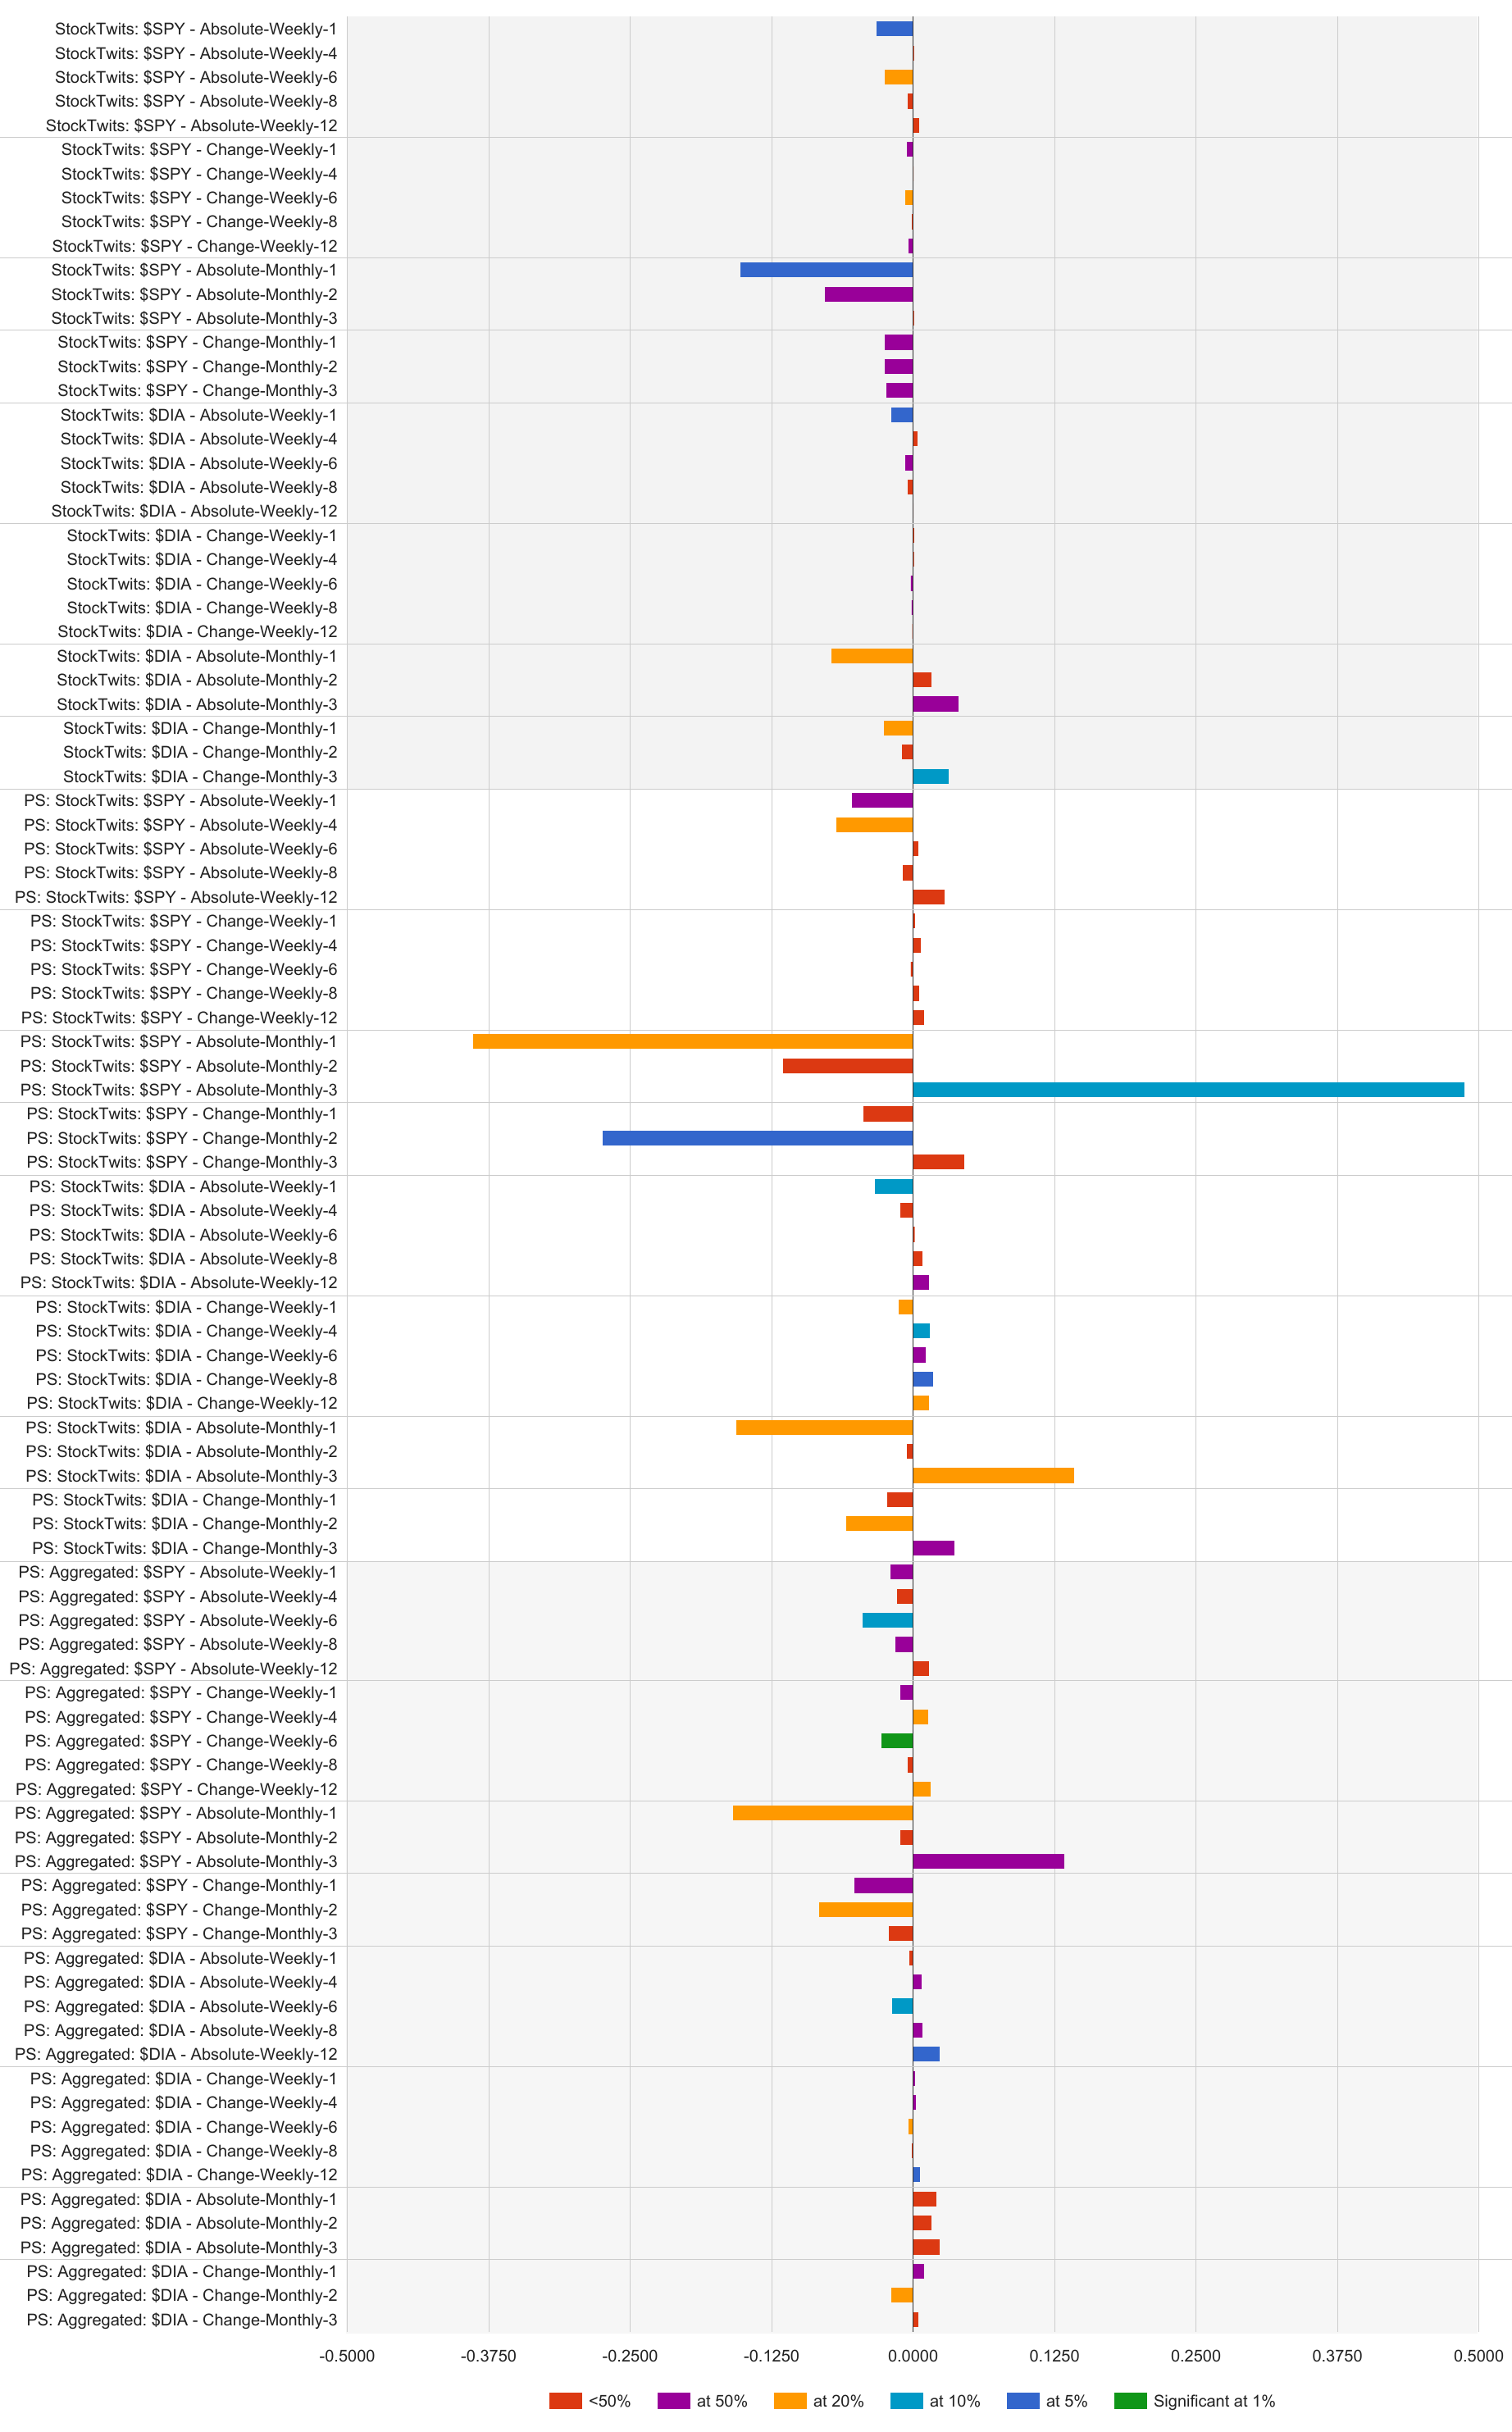
\includegraphics[width=.95\textwidth]{figures/sickExcelBars.png}
\caption{\label{fig:excelbars}Effect sizes of the regressions and their significance}
\end{figure}

\subsubsection{Economic Significance}
The effect sizes of most of our results are that 1\% change or increase of 1 in investor sentiment yields to sub 0.10\% change in stock returns. The exact magnitudes can be seen in Figure~\ref{fig:excelbars}. These results are similar to the results of Smales (2017) for large caps, Brown and Cliff (2002) for smaller companies and Fisher and Statman (2000) for individual investors sentiment on S\&P 500. There are no clear patterns in the magnitudes of our results and the results of past papers. Including the sentiment measures that we explored in our research, would therefore be a good addition to other tools when deciding on an investment, rather than a single decisive factor. The largest application of our findings are most suitable to quantitative trading, where it will help to fine tune the algorithms. 

\subsection{Recommendations}
Our aim was to investigate these new, modern sentiment measures and their relationship to subsequent stock returns. The services which gather and compile the sentiment measures (StockTwits and PsychSignal) create large datasets which are publicly available for people to use in their research or investment strategy. Investors can employ our findings in multiple ways. When constructing an algorithmic trading strategy, they can include a variable which tracks the sentiment measure either from PsychSignal or StockTwits and improve their predictive power of subsequent stock returns.

\subsection{Limitations and Future Research}
Since NLP processing and trading social networks such as StockTwits are fairly new concepts, we have analysed only the recent years (2014-2016) since this is the period for which the number of investor sentiment measures is sufficient to perform this type of research. This also prevented us from using a company level approach as desired from the start. As a proxy for returns of S\&P 500 index returns, we employed the S\&P 500 ETF \$SPY since this was the only data available to us on the research platform Quantopian where we accessed the PsychSignal databases. The velocity of the data is insufficient (so far!) to perform a company level (stock by stock) analysis for all S\&P 500 stocks on the effect of this type of investor sentiment on subsequent stock returns. When investigating the data, we have seen a huge growth over the recent years and we strongly believe that company level analysis will be available in the near future. This is also related to the decision to use aggregated data over weeks and months. Larger amounts of data will allow researchers to investigate these relationships on a day-to-day basis with sufficient data for either S\&P 500 or all stocks in NASDAQ or NYSE. We consider that shorter lags used in the upcoming research would bring more insights into how fast the social media investor sentiment can affect the subsequent stock returns.
\par
Furthermore, we tried to also test aggregating all daily sentiment (for all stock symbols) in StockTwits database and regressing this variable on Dow Jones Industrial Average and S\&P 500 indices. These tests did not yield any significant results and most of the p-values were higher than 0.90 for all lags. This big data approach is likely to become more relevant as more sentiment data will be generated by the users, both on Twitter and StockTwits.
\par
Regarding the absolute investor sentiment measures, some argue that causality in this measure is lowered as the effect size parameter may not be the correlation or regression of changes of investor sentiment on changes of stock returns, but may be the correlation or regression of the values of these variables at different points in time. This changes the quasi-experimental approach to a cross-sectional study over time, which means that causal inferences are not strictly implied.


\section{Acknowledgements}
Firstly, we wish to express our sincere thanks to Dr. Sarah Draus, assistant professor at the Finance Department of Rotterdam School of Management, for providing us with feedback and guiding us in the right direction during the process of writing the thesis. Special thanks to StockTwits for providing us access to their database. Lastly, we appreciate PsychSignal's work to create the NLP algorithm and make available sentiment data, and especially to Ernesto Ezequiel Perez from Quantopian for all his help and advice.

\bibliographystyle{apalike}
\bibliography{bibliography}

Baker, Malcolm, and Jeffrey Wurgler. "Investor sentiment in the stock market." The Journal of Economic \hspace*{8ex}Perspectives 21.2 (2007): 129-151.

Bollen, Johan, Huina Mao, and Xiaojun Zeng. "Twitter mood predicts the stock market." Journal of \hspace*{8ex}computational science 2.1 (2011): 1-8.

Brown, Gregory W. and Michael T. Cliff. "Investor Sentiment And The Near-Term Stock Market". \hspace*{8ex}Journal of Empirical Finance 11.1 (2004): 1-27.

Chen, Ray, and Marius Lazer. "Sentiment analysis of twitter feeds for the prediction of stock market \hspace*{8ex}movement." stanford. edu. Retrieved January 25 (2013): 2013.

Chui, Andy C.W., Titman, Sheridan and Wei, K.C. John, (2010), Individualism and Momentum around \hspace*{8ex}the World, Journal of Finance, 65, issue 1, p. 361-392, http://EconPapers.repec.org/RePEc:bla:jfi\\\hspace*{8ex}nan:v:65:y:2010:i:1:p:361-392.

Clarke, Roger G., and Meir Statman. "Bullish or bearish?."Financial Analysts Journal(1998): 63-72.

Dergiades, Theologos. "Do Investors’ Sentiment Dynamics Affect Stock Returns? Evidence From The \hspace*{8ex}US Economy".Economics Letters116.3 (2012): 404-407. Web.

Fisher, Kenneth L. and Meir Statman. "Investor Sentiment And Stock Returns". Financial Analysts \hspace*{8ex}Journal 56.2 (2000): 16-23.

Giot, Pierre. "Relationships between implied volatility indexes and stock index returns." The Journal of \hspace*{8ex}Portfolio Management 31.3 (2005): 92-100.

Hofstede, Geert. "Culture's recent consequences: Using dimension scores in theory and research." \hspace*{8ex}International Journal of cross cultural management 1.1 (2001): 11-17.

Lemmon, Michael, and Evgenia Portniaguina. "Consumer confidence and asset prices: Some empirical \hspace*{8ex}evidence." Review of Financial Studies 19.4 (2006): 1499-1529.

Liu, Shuming. "Investor Sentiment And Stock Market Liquidity". Journal of Behavioral Finance 16.1 \hspace*{8ex}(2015): 51-67. Web.

Rao, Tushar, and Saket Srivastava. "Analyzing stock market movements using twitter sentiment \\\hspace*{8ex}analysis." Proceedings of the 2012 International Conference on Advances in Social Networks \hspace*{8ex}Analysis and Mining (ASONAM 2012). IEEE Computer Society, 2012.

Simon, David P., and Roy A. Wiggins. "S\&P futures returns and contrary sentiment indicators." Journal \hspace*{8ex}of futures markets 21.5 (2001): 447-462.

Skuza, Michał, and Andrzej Romanowski. "Sentiment analysis of Twitter data within big data \\\hspace*{8ex}distributed environment for stock prediction." Computer Science and Information Systems \\\hspace*{8ex}(FedCSIS), 2015 Federated Conference on. IEEE, 2015.

Smales, L.A. "The Importance Of Fear: Investor Sentiment And Stock Market Returns".Applied Eco\\\hspace*{8ex}nomics(2017): 1-27. Web.

Solt, Michael E., and Meir Statman. "How useful is the sentiment index?."Financial Analysts Journal\\\hspace*{8ex}(1988): 45-55.

Tetlock, Paul C. "Giving content to investor sentiment: The role of media in the stock market." The \hspace*{8ex}Journal of Finance 62.3 (2007): 1139-1168.

Whaley, Robert E. "The investor fear gauge." The Journal of Portfolio Management 26.3 (2000): 12-17


\begin{landscape}
\newpage
\section{Appendix}

% Table generated by Excel2LaTeX from sheet 'appendix'
\begin{longtable}{ccccccrrrrr}
    \multicolumn{4}{l}{\textbf{Independent: Investors sentiment}} & \multicolumn{2}{c}{\textbf{Dependent: Stock returns}} & \multicolumn{2}{c}{} & \multicolumn{2}{c}{} &  \\
    \textbf{Name} & \textbf{Aggregate} & \textbf{Time-frame} & \textbf{Database} & \textbf{Name} & \textbf{Lag} & \multicolumn{1}{c}{\textbf{Slope}} & \multicolumn{2}{c}{\textbf{p-value}} & \multicolumn{2}{c}{\textbf{$R^2$}} \\
    \midrule
    \endhead
    \$SPY sentiment & Absolute & Weekly & StockTwits & \$SPY return & \textbf{1} & \textbf{-0.0328} & \multicolumn{2}{r}{\textbf{0.0368**}} & \multicolumn{2}{r}{\textbf{2.80\%}} \\
    \$SPY sentiment & Absolute & Weekly & StockTwits & \$SPY return & 4     & 0.0010 & \multicolumn{2}{r}{0.9515} & \multicolumn{2}{r}{0.00\%} \\
    \$SPY sentiment & Absolute & Weekly & StockTwits & \$SPY return & 6     & -0.0250 & \multicolumn{2}{r}{0.1069} & \multicolumn{2}{r}{1.68\%} \\
    \$SPY sentiment & Absolute & Weekly & StockTwits & \$SPY return & 8     & -0.0050 & \multicolumn{2}{r}{0.7466} & \multicolumn{2}{r}{0.07\%} \\
    \$SPY sentiment & Absolute & Weekly & StockTwits & \$SPY return & 12    & 0.0060 & \multicolumn{2}{r}{0.7026} & \multicolumn{2}{r}{0.09\%} \\
    \$SPY sentiment & Change & Weekly & StockTwits & \$SPY return & 1     & -0.0055 & \multicolumn{2}{r}{0.3271} & \multicolumn{2}{r}{0.63\%} \\
    \$SPY sentiment & Change & Weekly & StockTwits & \$SPY return & 4     & 0.0004 & \multicolumn{2}{r}{0.9379} & \multicolumn{2}{r}{0.00\%} \\
    \$SPY sentiment & Change & Weekly & StockTwits & \$SPY return & 6     & -0.0075 & \multicolumn{2}{r}{0.1744} & \multicolumn{2}{r}{1.20\%} \\
    \$SPY sentiment & Change & Weekly & StockTwits & \$SPY return & 8     & -0.0014 & \multicolumn{2}{r}{0.8050} & \multicolumn{2}{r}{0.04\%} \\
    \$SPY sentiment & Change & Weekly & StockTwits & \$SPY return & 12    & -0.0040 & \multicolumn{2}{r}{0.4671} & \multicolumn{2}{r}{0.35\%} \\
    \$SPY sentiment & Absolute & Monthly & StockTwits & \$SPY return & \textbf{1} & \textbf{-0.1531} & \multicolumn{2}{r}{\textbf{0.0479**}} & \multicolumn{2}{r}{\textbf{11.02\%}} \\
    \$SPY sentiment & Absolute & Monthly & StockTwits & \$SPY return & 2     & -0.0786 & \multicolumn{2}{r}{0.3182} & \multicolumn{2}{r}{2.93\%} \\
    \$SPY sentiment & Absolute & Monthly & StockTwits & \$SPY return & 3     & 0.0010 & \multicolumn{2}{r}{0.9903} & \multicolumn{2}{r}{0.00\%} \\
    \$SPY sentiment & Change & Monthly & StockTwits & \$SPY return & 1     & -0.0253 & \multicolumn{2}{r}{0.3579} & \multicolumn{2}{r}{2.57\%} \\
    \$SPY sentiment & Change & Monthly & StockTwits & \$SPY return & 2     & -0.0252 & \multicolumn{2}{r}{0.3669} & \multicolumn{2}{r}{2.47\%} \\
    \$SPY sentiment & Change & Monthly & StockTwits & \$SPY return & 3     & -0.0241 & \multicolumn{2}{r}{0.3910} & \multicolumn{2}{r}{2.24\%} \\
    \$DIA sentiment & Absolute & Weekly & StockTwits & \$DIA return & \textbf{1} & \textbf{-0.0199} & \multicolumn{2}{r}{\textbf{0.0283**}} & \multicolumn{2}{r}{\textbf{3.08\%}} \\
    \$DIA sentiment & Absolute & Weekly & StockTwits & \$DIA return & 4     & 0.0043 & \multicolumn{2}{r}{0.6287} & \multicolumn{2}{r}{0.15\%} \\
    \$DIA sentiment & Absolute & Weekly & StockTwits & \$DIA return & 6     & -0.0073 & \multicolumn{2}{r}{0.4135} & \multicolumn{2}{r}{0.43\%} \\
    \$DIA sentiment & Absolute & Weekly & StockTwits & \$DIA return & 8     & -0.0048 & \multicolumn{2}{r}{0.5929} & \multicolumn{2}{r}{0.19\%} \\
    \$DIA sentiment & Absolute & Weekly & StockTwits & \$DIA return & 12    & 0.0001 & \multicolumn{2}{r}{0.9870} & \multicolumn{2}{r}{0.00\%} \\
    \$DIA sentiment & Change & Weekly & StockTwits & \$DIA return & 1     & 0.0011 & \multicolumn{2}{r}{0.6011} & \multicolumn{2}{r}{0.18\%} \\
    \$DIA sentiment & Change & Weekly & StockTwits & \$DIA return & 4     & 0.0009 & \multicolumn{2}{r}{0.6478} & \multicolumn{2}{r}{0.14\%} \\
    \$DIA sentiment & Change & Weekly & StockTwits & \$DIA return & 6     & -0.0024 & \multicolumn{2}{r}{0.2290} & \multicolumn{2}{r}{0.94\%} \\
    \$DIA sentiment & Change & Weekly & StockTwits & \$DIA return & 8     & -0.0015 & \multicolumn{2}{r}{0.4488} & \multicolumn{2}{r}{0.38\%} \\
    \$DIA sentiment & Change & Weekly & StockTwits & \$DIA return & 12    & -0.0007 & \multicolumn{2}{r}{0.7261} & \multicolumn{2}{r}{0.08\%} \\
    \$DIA sentiment & Absolute & Monthly & StockTwits & \$DIA return & 1     & -0.0728 & \multicolumn{2}{r}{0.1483} & \multicolumn{2}{r}{6.05\%} \\
    \$DIA sentiment & Absolute & Monthly & StockTwits & \$DIA return & 2     & 0.0166 & \multicolumn{2}{r}{0.7470} & \multicolumn{2}{r}{0.31\%} \\
    \$DIA sentiment & Absolute & Monthly & StockTwits & \$DIA return & 3     & 0.0403 & \multicolumn{2}{r}{0.4364} & \multicolumn{2}{r}{1.79\%} \\
    \$DIA sentiment & Change & Monthly & StockTwits & \$DIA return & 1     & -0.0258 & \multicolumn{2}{r}{0.1229} & \multicolumn{2}{r}{7.06\%} \\
    \$DIA sentiment & Change & Monthly & StockTwits & \$DIA return & 2     & -0.0102 & \multicolumn{2}{r}{0.5588} & \multicolumn{2}{r}{1.05\%} \\
    \$DIA sentiment & Change & Monthly & StockTwits & \$DIA return & \textbf{3} & \textbf{0.0320} & \multicolumn{2}{r}{\textbf{0.0612*}} & \multicolumn{2}{r}{\textbf{10.22\%}} \\
    \$SPY sentiment & Absolute & Weekly & PS:StockTwits & \$SPY return & 1     & -0.0543 & \multicolumn{2}{r}{0.2395} & \multicolumn{2}{r}{0.89\%} \\
    \$SPY sentiment & Absolute & Weekly & PS:StockTwits & \$SPY return & 4     & -0.0682 & \multicolumn{2}{r}{0.1368} & \multicolumn{2}{r}{1.42\%} \\
    \$SPY sentiment & Absolute & Weekly & PS:StockTwits & \$SPY return & 6     & 0.0048 & \multicolumn{2}{r}{0.9175} & \multicolumn{2}{r}{0.01\%} \\
    \$SPY sentiment & Absolute & Weekly & PS:StockTwits & \$SPY return & 8     & -0.0092 & \multicolumn{2}{r}{0.8404} & \multicolumn{2}{r}{0.03\%} \\
    \$SPY sentiment & Absolute & Weekly & PS:StockTwits & \$SPY return & 12    & 0.0284 & \multicolumn{2}{r}{0.5315} & \multicolumn{2}{r}{0.25\%} \\
    \$SPY sentiment & Change & Weekly & PS:StockTwits & \$SPY return & 1     & 0.0022 & \multicolumn{2}{r}{0.9227} & \multicolumn{2}{r}{0.01\%} \\
    \$SPY sentiment & Change & Weekly & PS:StockTwits & \$SPY return & 4     & 0.0073 & \multicolumn{2}{r}{0.7413} & \multicolumn{2}{r}{0.07\%} \\
    \$SPY sentiment & Change & Weekly & PS:StockTwits & \$SPY return & 6     & -0.0025 & \multicolumn{2}{r}{0.9122} & \multicolumn{2}{r}{0.01\%} \\
    \$SPY sentiment & Change & Weekly & PS:StockTwits & \$SPY return & 8     & 0.0061 & \multicolumn{2}{r}{0.7799} & \multicolumn{2}{r}{0.05\%} \\
    \$SPY sentiment & Change & Weekly & PS:StockTwits & \$SPY return & 12    & 0.0101 & \multicolumn{2}{r}{0.6425} & \multicolumn{2}{r}{0.14\%} \\
    \$SPY sentiment & Absolute & Monthly & PS:StockTwits & \$SPY return & 1     & -0.3891 & \multicolumn{2}{r}{0.1498} & \multicolumn{2}{r}{6.00\%} \\
    \$SPY sentiment & Absolute & Monthly & PS:StockTwits & \$SPY return & 2     & -0.1150 & \multicolumn{2}{r}{0.6709} & \multicolumn{2}{r}{0.54\%} \\
    \$SPY sentiment & Absolute & Monthly & PS:StockTwits & \$SPY return & \textbf{3} & \textbf{0.4874} & \multicolumn{2}{r}{\textbf{0.0661*}} & \multicolumn{2}{r}{\textbf{9.59\%}} \\
    \$SPY sentiment & Change & Monthly & PS:StockTwits & \$SPY return & 1     & -0.0441 & \multicolumn{2}{r}{0.7381} & \multicolumn{2}{r}{0.34\%} \\
    \$SPY sentiment & Change & Monthly & PS:StockTwits & \$SPY return & \textbf{2} & \textbf{-0.2744} & \multicolumn{2}{r}{\textbf{0.0335**}} & \multicolumn{2}{r}{\textbf{12.98\%}} \\
    \$SPY sentiment & Change & Monthly & PS:StockTwits & \$SPY return & 3     & 0.0453 & \multicolumn{2}{r}{0.7349} & \multicolumn{2}{r}{0.35\%} \\
    \$DIA sentiment & Absolute & Weekly & PS:StockTwits & \$DIA return & \textbf{1} & \textbf{-0.0339} & \multicolumn{2}{r}{\textbf{0.0747*}} & \multicolumn{2}{r}{\textbf{2.03\%}} \\
    \$DIA sentiment & Absolute & Weekly & PS:StockTwits & \$DIA return & 4     & -0.0119 & \multicolumn{2}{r}{0.5268} & \multicolumn{2}{r}{0.26\%} \\
    \$DIA sentiment & Absolute & Weekly & PS:StockTwits & \$DIA return & 6     & 0.0015 & \multicolumn{2}{r}{0.9369} & \multicolumn{2}{r}{0.00\%} \\
    \$DIA sentiment & Absolute & Weekly & PS:StockTwits & \$DIA return & 8     & 0.0085 & \multicolumn{2}{r}{0.6515} & \multicolumn{2}{r}{0.13\%} \\
    \$DIA sentiment & Absolute & Weekly & PS:StockTwits & \$DIA return & 12    & 0.0147 & \multicolumn{2}{r}{0.4326} & \multicolumn{2}{r}{0.40\%} \\
    \$DIA sentiment & Change & Weekly & PS:StockTwits & \$DIA return & 1     & -0.0132 & \multicolumn{2}{r}{0.1462} & \multicolumn{2}{r}{1.37\%} \\
    \$DIA sentiment & Change & Weekly & PS:StockTwits & \$DIA return & \textbf{4} & \textbf{0.0149} & \multicolumn{2}{r}{\textbf{0.0970*}} & \multicolumn{2}{r}{\textbf{1.78\%}} \\
    \$DIA sentiment & Change & Weekly & PS:StockTwits & \$DIA return & 6     & 0.0115 & \multicolumn{2}{r}{0.2070} & \multicolumn{2}{r}{1.03\%} \\
    \$DIA sentiment & Change & Weekly & PS:StockTwits & \$DIA return & \textbf{8} & \textbf{0.0183} & \multicolumn{2}{r}{\textbf{0.0402**}} & \multicolumn{2}{r}{\textbf{2.71\%}} \\
    \$DIA sentiment & Change & Weekly & PS:StockTwits & \$DIA return & 12    & 0.0146 & \multicolumn{2}{r}{0.1022} & \multicolumn{2}{r}{1.73\%} \\
    \$DIA sentiment & Absolute & Monthly & PS:StockTwits & \$DIA return & 1     & -0.1565 & \multicolumn{2}{r}{0.1298} & \multicolumn{2}{r}{6.62\%} \\
    \$DIA sentiment & Absolute & Monthly & PS:StockTwits & \$DIA return & 2     & -0.0059 & \multicolumn{2}{r}{0.9554} & \multicolumn{2}{r}{0.01\%} \\
    \$DIA sentiment & Absolute & Monthly & PS:StockTwits & \$DIA return & 3     & 0.1429 & \multicolumn{2}{r}{0.1732} & \multicolumn{2}{r}{5.39\%} \\
    \$DIA sentiment & Change & Monthly & PS:StockTwits & \$DIA return & 1     & -0.0235 & \multicolumn{2}{r}{0.6043} & \multicolumn{2}{r}{0.82\%} \\
    \$DIA sentiment & Change & Monthly & PS:StockTwits & \$DIA return & 2     & -0.0597 & \multicolumn{2}{r}{0.1922} & \multicolumn{2}{r}{5.10\%} \\
    \$DIA sentiment & Change & Monthly & PS:StockTwits & \$DIA return & 3     & 0.0366 & \multicolumn{2}{r}{0.4304} & \multicolumn{2}{r}{1.89\%} \\
    \$SPY sentiment & Absolute & Weekly & PS:Aggregated & \$SPY return & 1     & -0.0206 & \multicolumn{2}{r}{0.3889} & \multicolumn{2}{r}{0.48\%} \\
    \$SPY sentiment & Absolute & Weekly & PS:Aggregated & \$SPY return & 4     & -0.0145 & \multicolumn{2}{r}{0.5429} & \multicolumn{2}{r}{0.24\%} \\
    \$SPY sentiment & Absolute & Weekly & PS:Aggregated & \$SPY return & \textbf{6} & \textbf{-0.0448} & \multicolumn{2}{r}{\textbf{0.0599*}} & \multicolumn{2}{r}{\textbf{2.27\%}} \\
    \$SPY sentiment & Absolute & Weekly & PS:Aggregated & \$SPY return & 8     & -0.0163 & \multicolumn{2}{r}{0.4905} & \multicolumn{2}{r}{0.31\%} \\
    \$SPY sentiment & Absolute & Weekly & PS:Aggregated & \$SPY return & 12    & 0.0145 & \multicolumn{2}{r}{0.5397} & \multicolumn{2}{r}{0.24\%} \\
    \$SPY sentiment & Change & Weekly & PS:Aggregated & \$SPY return & 1     & -0.0114 & \multicolumn{2}{r}{0.2809} & \multicolumn{2}{r}{0.75\%} \\
    \$SPY sentiment & Change & Weekly & PS:Aggregated & \$SPY return & 4     & 0.0138 & \multicolumn{2}{r}{0.1882} & \multicolumn{2}{r}{1.12\%} \\
    \$SPY sentiment & Change & Weekly & PS:Aggregated & \$SPY return & \textbf{6} & \textbf{-0.0280} & \multicolumn{2}{r}{\textbf{0.0075***}} & \multicolumn{2}{r}{\textbf{4.54\%}} \\
    \$SPY sentiment & Change & Weekly & PS:Aggregated & \$SPY return & 8     & -0.0049 & \multicolumn{2}{r}{0.6362} & \multicolumn{2}{r}{0.15\%} \\
    \$SPY sentiment & Change & Weekly & PS:Aggregated & \$SPY return & 12    & 0.0158 & \multicolumn{2}{r}{0.1289} & \multicolumn{2}{r}{1.49\%} \\
    \$SPY sentiment & Absolute & Monthly & PS:Aggregated & \$SPY return & 1     & -0.1593 & \multicolumn{2}{r}{0.1667} & \multicolumn{2}{r}{5.55\%} \\
    \$SPY sentiment & Absolute & Monthly & PS:Aggregated & \$SPY return & 2     & -0.0115 & \multicolumn{2}{r}{0.9209} & \multicolumn{2}{r}{0.03\%} \\
    \$SPY sentiment & Absolute & Monthly & PS:Aggregated & \$SPY return & 3     & 0.1342 & \multicolumn{2}{r}{0.2416} & \multicolumn{2}{r}{4.01\%} \\
    \$SPY sentiment & Change & Monthly & PS:Aggregated & \$SPY return & 1     & -0.0525 & \multicolumn{2}{r}{0.3572} & \multicolumn{2}{r}{2.57\%} \\
    \$SPY sentiment & Change & Monthly & PS:Aggregated & \$SPY return & 2     & -0.0830 & \multicolumn{2}{r}{0.1463} & \multicolumn{2}{r}{6.28\%} \\
    \$SPY sentiment & Change & Monthly & PS:Aggregated & \$SPY return & 3     & -0.0214 & \multicolumn{2}{r}{0.7122} & \multicolumn{2}{r}{0.42\%} \\
    \$DIA sentiment & Absolute & Weekly & PS:Aggregated & \$DIA return & 1     & -0.0036 & \multicolumn{2}{r}{0.7240} & \multicolumn{2}{r}{0.08\%} \\
    \$DIA sentiment & Absolute & Weekly & PS:Aggregated & \$DIA return & 4     & 0.0082 & \multicolumn{2}{r}{0.4079} & \multicolumn{2}{r}{0.44\%} \\
    \$DIA sentiment & Absolute & Weekly & PS:Aggregated & \$DIA return & \textbf{6} & \textbf{-0.0187} & \multicolumn{2}{r}{\textbf{0.0628*}} & \multicolumn{2}{r}{\textbf{2.22\%}} \\
    \$DIA sentiment & Absolute & Weekly & PS:Aggregated & \$DIA return & 8     & 0.0088 & \multicolumn{2}{r}{0.3790} & \multicolumn{2}{r}{0.50\%} \\
    \$DIA sentiment & Absolute & Weekly & PS:Aggregated & \$DIA return & \textbf{12} & \textbf{0.0239} & \multicolumn{2}{r}{\textbf{0.0152**}} & \multicolumn{2}{r}{\textbf{3.74\%}} \\
    \$DIA sentiment & Change & Weekly & PS:Aggregated & \$DIA return & 1     & 0.0023 & \multicolumn{2}{r}{0.4316} & \multicolumn{2}{r}{0.40\%} \\
    \$DIA sentiment & Change & Weekly & PS:Aggregated & \$DIA return & 4     & 0.0032 & \multicolumn{2}{r}{0.2553} & \multicolumn{2}{r}{0.84\%} \\
    \$DIA sentiment & Change & Weekly & PS:Aggregated & \$DIA return & 6     & -0.0041 & \multicolumn{2}{r}{0.1609} & \multicolumn{2}{r}{1.27\%} \\
    \$DIA sentiment & Change & Weekly & PS:Aggregated & \$DIA return & 8     & -0.0011 & \multicolumn{2}{r}{0.6953} & \multicolumn{2}{r}{0.10\%} \\
    \$DIA sentiment & Change & Weekly & PS:Aggregated & \$DIA return & \textbf{12} & \textbf{0.0068} & \multicolumn{2}{r}{\textbf{0.0168**}} & \multicolumn{2}{r}{\textbf{3.66\%}} \\
    \$DIA sentiment & Absolute & Monthly & PS:Aggregated & \$DIA return & 1     & 0.0209 & \multicolumn{2}{r}{0.6325} & \multicolumn{2}{r}{0.68\%} \\
    \$DIA sentiment & Absolute & Monthly & PS:Aggregated & \$DIA return & 2     & 0.0165 & \multicolumn{2}{r}{0.7075} & \multicolumn{2}{r}{0.42\%} \\
    \$DIA sentiment & Absolute & Monthly & PS:Aggregated & \$DIA return & 3     & 0.0241 & \multicolumn{2}{r}{0.5860} & \multicolumn{2}{r}{0.88\%} \\
    \$DIA sentiment & Change & Monthly & PS:Aggregated & \$DIA return & 1     & 0.0101 & \multicolumn{2}{r}{0.4530} & \multicolumn{2}{r}{1.72\%} \\
    \$DIA sentiment & Change & Monthly & PS:Aggregated & \$DIA return & 2     & -0.0192 & \multicolumn{2}{r}{0.1586} & \multicolumn{2}{r}{5.93\%} \\
    \$DIA sentiment & Change & Monthly & PS:Aggregated & \$DIA return & 3     & 0.0053 & \multicolumn{2}{r}{0.7058} & \multicolumn{2}{r}{0.44\%} \\
    
    %\caption{Add caption}
	\label{tab:appendix}%
    \end{longtable}%
 
  



% Table generated by Excel2LaTeX from sheet 'Sheet1'
\begin{table}[htbp]
  \centering
  \caption{Results Correlation of modern sentiment measures}
    \begin{tabular}{cccccccccc}
    \multicolumn{3}{c}{\textbf{VAR1}} &       & \multicolumn{3}{c}{\textbf{VAR2}} &       & \multicolumn{2}{c}{\textbf{RESULTS}} \\
    \midrule
    \textbf{Name} & \textbf{Period} & \textbf{Database} &       & \textbf{Name} & \textbf{Period} & \textbf{Database} &       & \textbf{Coeff} & \textbf{p-value} \\
    \midrule
    SPY sentiment & Weekly & PS:Stocktwits  &       & SPY sentiment & Weekly & StockTwits     &       & \textbf{0.5533} & \textbf{0.0000***} \\
    SPY sentiment & Weekly & PS:Stocktwits  &       & SPY sentiment & Weekly & PS:Aggregated  &       & \textbf{0.5321} & \textbf{0.0000***} \\
    SPY sentiment & Weekly & StockTwits     &       & SPY sentiment & Weekly & PS:Aggregated  &       & \textbf{0.2786} & \textbf{0.0004***} \\
    DIA sentiment & Weekly & PS:Stocktwits  &       & DIA sentiment & Weekly & PS:Stocktwits  &       & \textbf{0.5708} & \textbf{0.0000***} \\
    DIA sentiment & Weekly & PS:Stocktwits  &       & DIA sentiment & Weekly & PS:Aggregated  &       & \textbf{0.4200} & \textbf{0.0000***} \\
    DIA sentiment & Weekly & StockTwits     &       & DIA sentiment & Weekly & PS:Aggregated  &       & \textbf{0.2136} & \textbf{0.0072***} \\
    SPY sentiment & Weekly & PS:Aggregated  &       & DIA sentiment & Weekly & PS:Aggregated  &       & \textbf{0.3987} & \textbf{0.0000***} \\
    SPY sentiment & Weekly & StockTwits     &       & DIA sentiment & Weekly & StockTwits     &       & \textbf{0.3009} & \textbf{0.0001***} \\
    SPY sentiment & Weekly & PS:Stocktwits  &       & DIA sentiment & Weekly & PS:Stocktwits  &       & \textbf{0.6164} & \textbf{0.0000***} \\
    SPY sentiment & Monthly & PS:Stocktwits &       & SPY sentiment & Monthly & StockTwits    &       & \textbf{0.4887} & \textbf{0.0025***} \\
    SPY sentiment & Monthly & PS:Stocktwits &       & SPY sentiment & Monthly & PS:Aggregated &       & \textbf{0.6714} & \textbf{0.0000***} \\
    SPY sentiment & Monthly & StockTwits    &       & SPY sentiment & Monthly & PS:Aggregated &       & \textbf{0.4106} & \textbf{0.0129**} \\
    DIA sentiment & Monthly & PS:Stocktwits &       & DIA sentiment & Monthly & StockTwits    &       & \textbf{0.6472} & \textbf{0.0000***} \\
    DIA sentiment & Monthly & PS:Stocktwits &       & DIA sentiment & Monthly & PS:Aggregated &       & \textbf{0.6043} & \textbf{0.0001***} \\
    DIA sentiment & Monthly & StockTwits    &       & DIA sentiment & Monthly & PS:Aggregated &       & 0.2553          & 0.1329 \\
    SPY sentiment & Monthly & PS:Aggregated &       & DIA sentiment & Monthly & PS:Aggregated &       & \textbf{0.4270} & \textbf{0.0094***} \\
    SPY sentiment & Monthly & StockTwits    &       & DIA sentiment & Monthly & StockTwits    &       & 0.2671          & 0.1153 \\
    SPY sentiment & Monthly & PS:Stocktwits &       & DIA sentiment & Monthly & PS:Stocktwits &       & \textbf{0.7233} & \textbf{0.0000***} \\
    \end{tabular}%
  \label{tab:appendix2}%
\end{table}%


\end{landscape}


\end{document}